% !TeX spellcheck = en_GB
\documentclass[abstract,toc,los,lof,english,10pt,glossary,acronyms]{jluthesis}

\usepackage{gnuplottex}
\usepackage{gnuplot-lua-tikz}
\usepackage{listings}
\usepackage{float}
\newfloat{lstfloat}{tb}{lop}
\floatname{lstfloat}{Listing}

\usepackage{textgreek}
\usepackage{caption}
\usepackage{subcaption}
\renewcommand\thesubfigure{-\arabic{subfigure}}


\usepgfplotslibrary{fillbetween}

\usepackage{pdfpages}
\newacronym{eas}{EAS}{Extensive Air Showers}
\newacronym{uhecr}{UHECR}{Ultra High Energy Cosmic Radiation}
\newacronym{sipm}{SiPM}{Silicon Photomultiplier}
\newacronym{adc}{ADC}{Analog Digital Converter}
\newacronym{enu}{ENU}{East, North Up}
\newacronym{com}{COM}{center of mass}
\newacronym{csda}{CSDA}{continuous-slowing-down approximation}
\newacronym{gzkl}{GZK-Limit}{Greisen–Zatsepin–Kuzmin limit}
\newglossaryentry{hadron} {name=hadron, description={subatomic particle affected by the strong interaction}}
\newglossaryentry{nucleus} {name=nucleus, plural=nuclei, description={Center of an atom}}
\bibliography{data/thesis.bib}

\topic{Real-time data analysis of a distributed muon detector network for cosmic shower detection and reconstruction}
\title[Bachelor Thesis]{Bachelor Thesis}
\author[Daniel Treffenstädt]{Daniel J.S. Treffenstädt}
\matnr{6067797}
\reviewer{Prof. Dr. Kai-Thomas Brinkmann\\apl. Prof. Dr. Sören Lange}
\supervisor{Dr. Hans-Georg Zaunick}



\begin{document}
\tikzstyle{networknode} = [draw, circle, node distance=0.5cm]

\pgfdeclaredecoration{discontinuity}{start}{
	\state{start}[width=0.5\pgfdecoratedinputsegmentremainingdistance-0.5\pgfdecorationsegmentlength,next state=first wave]
	{}
	\state{first wave}[width=\pgfdecorationsegmentlength, next state=second wave]
	{
		\pgfpathlineto{\pgfpointorigin}
		\pgfpathmoveto{\pgfqpoint{0pt}{\pgfdecorationsegmentamplitude}}
		\pgfpathcurveto
		{\pgfpoint{-0.25*\pgfmetadecorationsegmentlength}{0.75\pgfdecorationsegmentamplitude}}
		{\pgfpoint{-0.25*\pgfmetadecorationsegmentlength}{0.25\pgfdecorationsegmentamplitude}}
		{\pgfpoint{0pt}{0pt}}
		\pgfpathcurveto
		{\pgfpoint{0.25*\pgfmetadecorationsegmentlength}{-0.25\pgfdecorationsegmentamplitude}}
		{\pgfpoint{0.25*\pgfmetadecorationsegmentlength}{-0.75\pgfdecorationsegmentamplitude}}
		{\pgfpoint{0pt}{-\pgfdecorationsegmentamplitude}}
	}
	\state{second wave}[width=0pt, next state=do nothing]
	{
		\pgfpathmoveto{\pgfqpoint{0pt}{\pgfdecorationsegmentamplitude}}
		\pgfpathcurveto
		{\pgfpoint{-0.25*\pgfmetadecorationsegmentlength}{0.75\pgfdecorationsegmentamplitude}}
		{\pgfpoint{-0.25*\pgfmetadecorationsegmentlength}{0.25\pgfdecorationsegmentamplitude}}
		{\pgfpoint{0pt}{0pt}}
		\pgfpathcurveto
		{\pgfpoint{0.25*\pgfmetadecorationsegmentlength}{-0.25\pgfdecorationsegmentamplitude}}
		{\pgfpoint{0.25*\pgfmetadecorationsegmentlength}{-0.75\pgfdecorationsegmentamplitude}}
		{\pgfpoint{0pt}{-\pgfdecorationsegmentamplitude}}
		\pgfpathmoveto{\pgfpointorigin}
	}
	\state{do nothing}[width=\pgfdecorationsegmentlength,next state=do nothing]{
		\pgfpathlineto{\pgfpointdecoratedinputsegmentlast}
	}
	\state{final}
	{
		\pgfpathlineto{\pgfpointdecoratedpathlast}
	}
}

	
\makebeginning{
	Extensive Air Showers produced by ultra high energy cosmic radiation are still an active area of research. Due to the low number of such events collecting statistics requires a lot of time. Different approaches to collecting data about these events can be taken, one approach is the usage of a distributed network of low-cost particle detectors which can be operated by persons outside the university environment to cover a maximum area without the need for large investments.
	
	In this thesis, a method is developed to perform real-time analysis for a network of low-cost plastic scintillator detectors. This network consists of small scintillator detectors with silicon Photomultiplier units which are attached to a Raspberry-Pi computer. Those detection units are located throughout Germany and send their data to a server where it is continuously monitored for coincidences.
	
	An approach to reconstructing the possible incident direction of the primary particle as well as an approximation for plausible energies is presented.
}
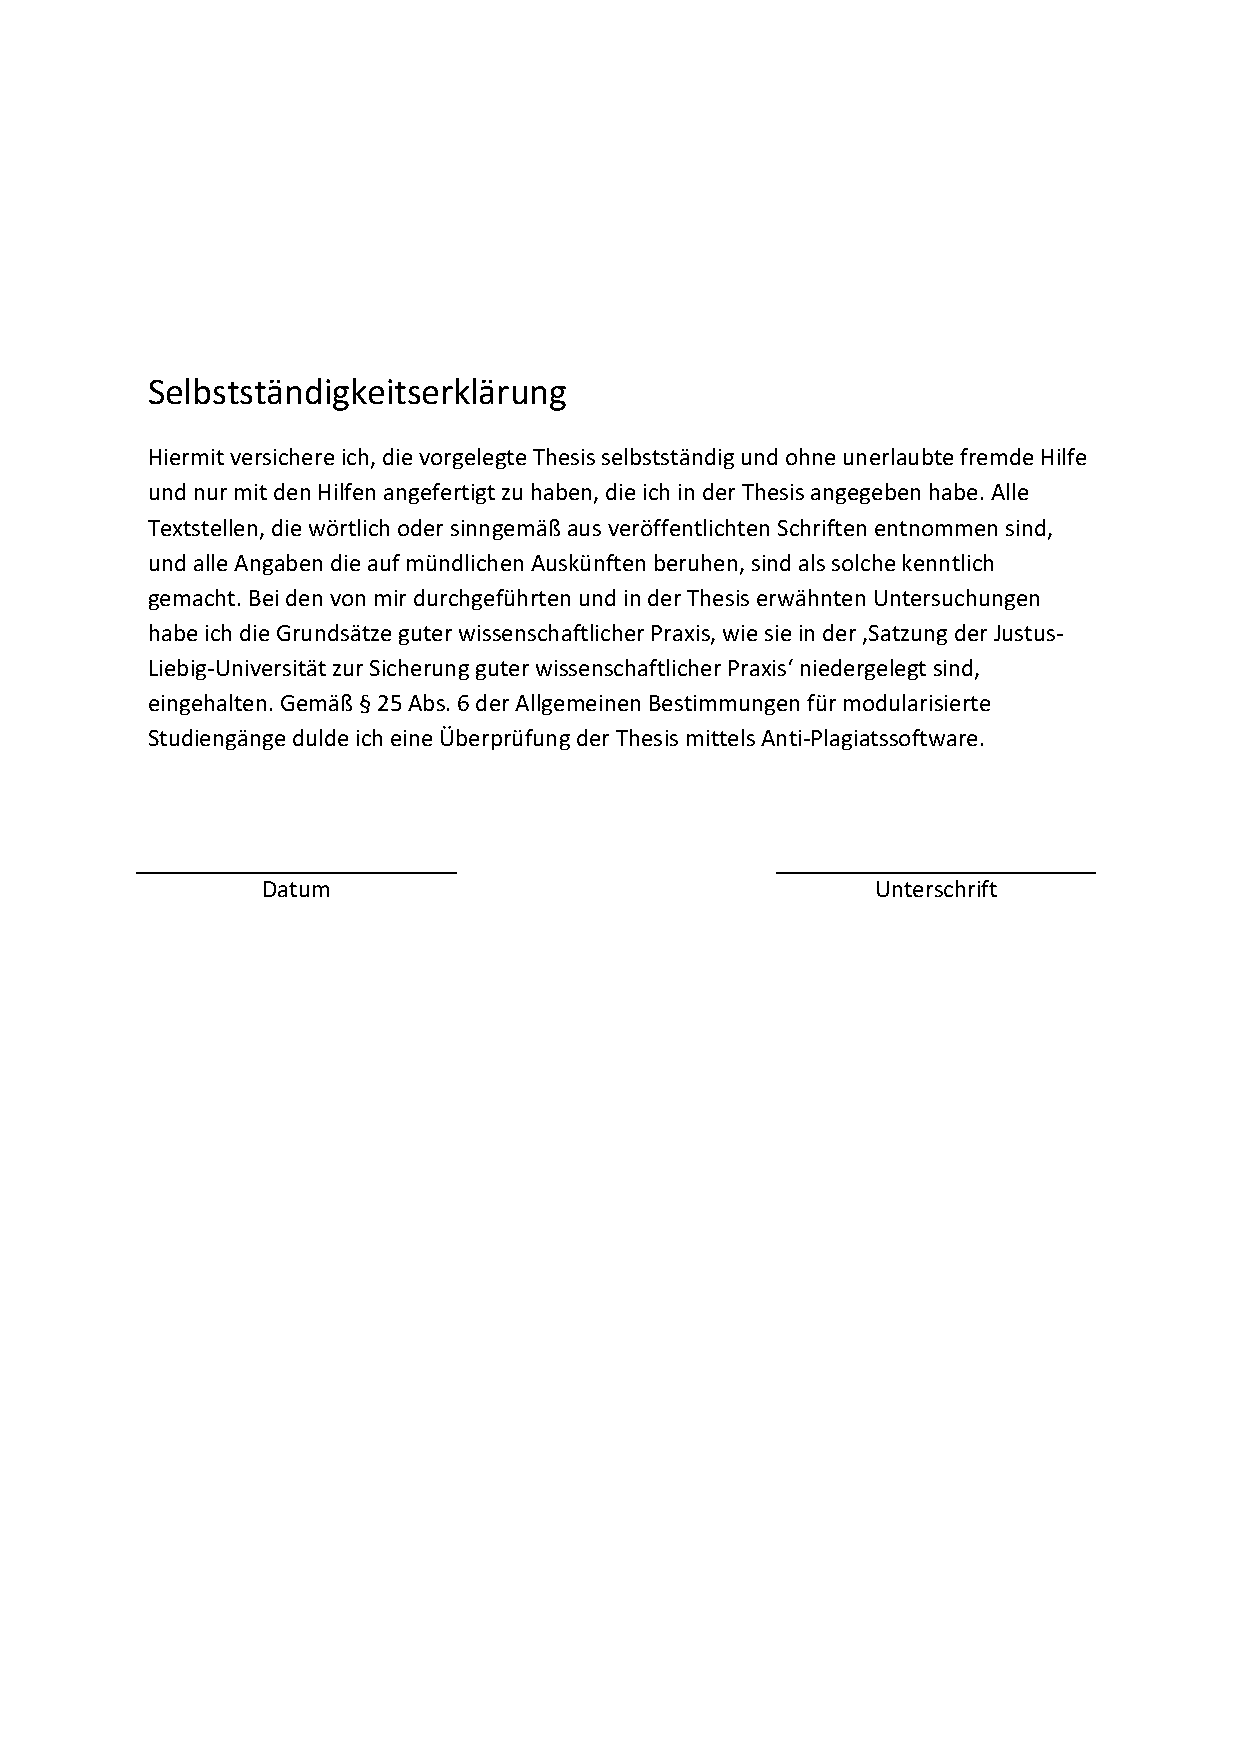
\includepdf[noautoscale=true, width=\paperwidth]{data/selbststaendigkeit.pdf}


\section{Introduction}
\subsection{Cosmic Radiation}
\acrfull{uhecr} is cosmic radiation with energy in the range of $10^{18}$\,eV to $10^{20}$\,eV.\footnote{The energy unit eV(Electron-Volt) describes the kinetic energy a unit charge holds after being accelerated through an electric field for 1V. It is equivalent to $1.602176634\cdot10^{-19}\,\text{J}$.}
Cosmic radiation has been discovered in 1912 by Viktor Hess by performing measurements with three electrometers in a balloon flight. He measured the energy flux in the atmosphere and showed that it increased with altitude. This is explained by secondary particles which are produced through the interaction of primary cosmic radiation with the atmosphere. The cosmic radiation is produced by many different sources, one of which is our sun. The sun however only produces cosmic radiation up to a few hundred MeV of energy through coronal mass ejections and other processes and so is not contributing to \acrshort{uhecr}.

Higher energy sources include other stars, supernovae or accretion disks around black holes. Though the production mechanism for the highest energy sources are still not fully understood and no sources have been identified definitively. Current research at the Pierre-Auger observatory shows an anisotropy in the arrival directions and suggests various sources \cite{fargion2018ultra}.
\begin{figure}[ht!]
	\centering
	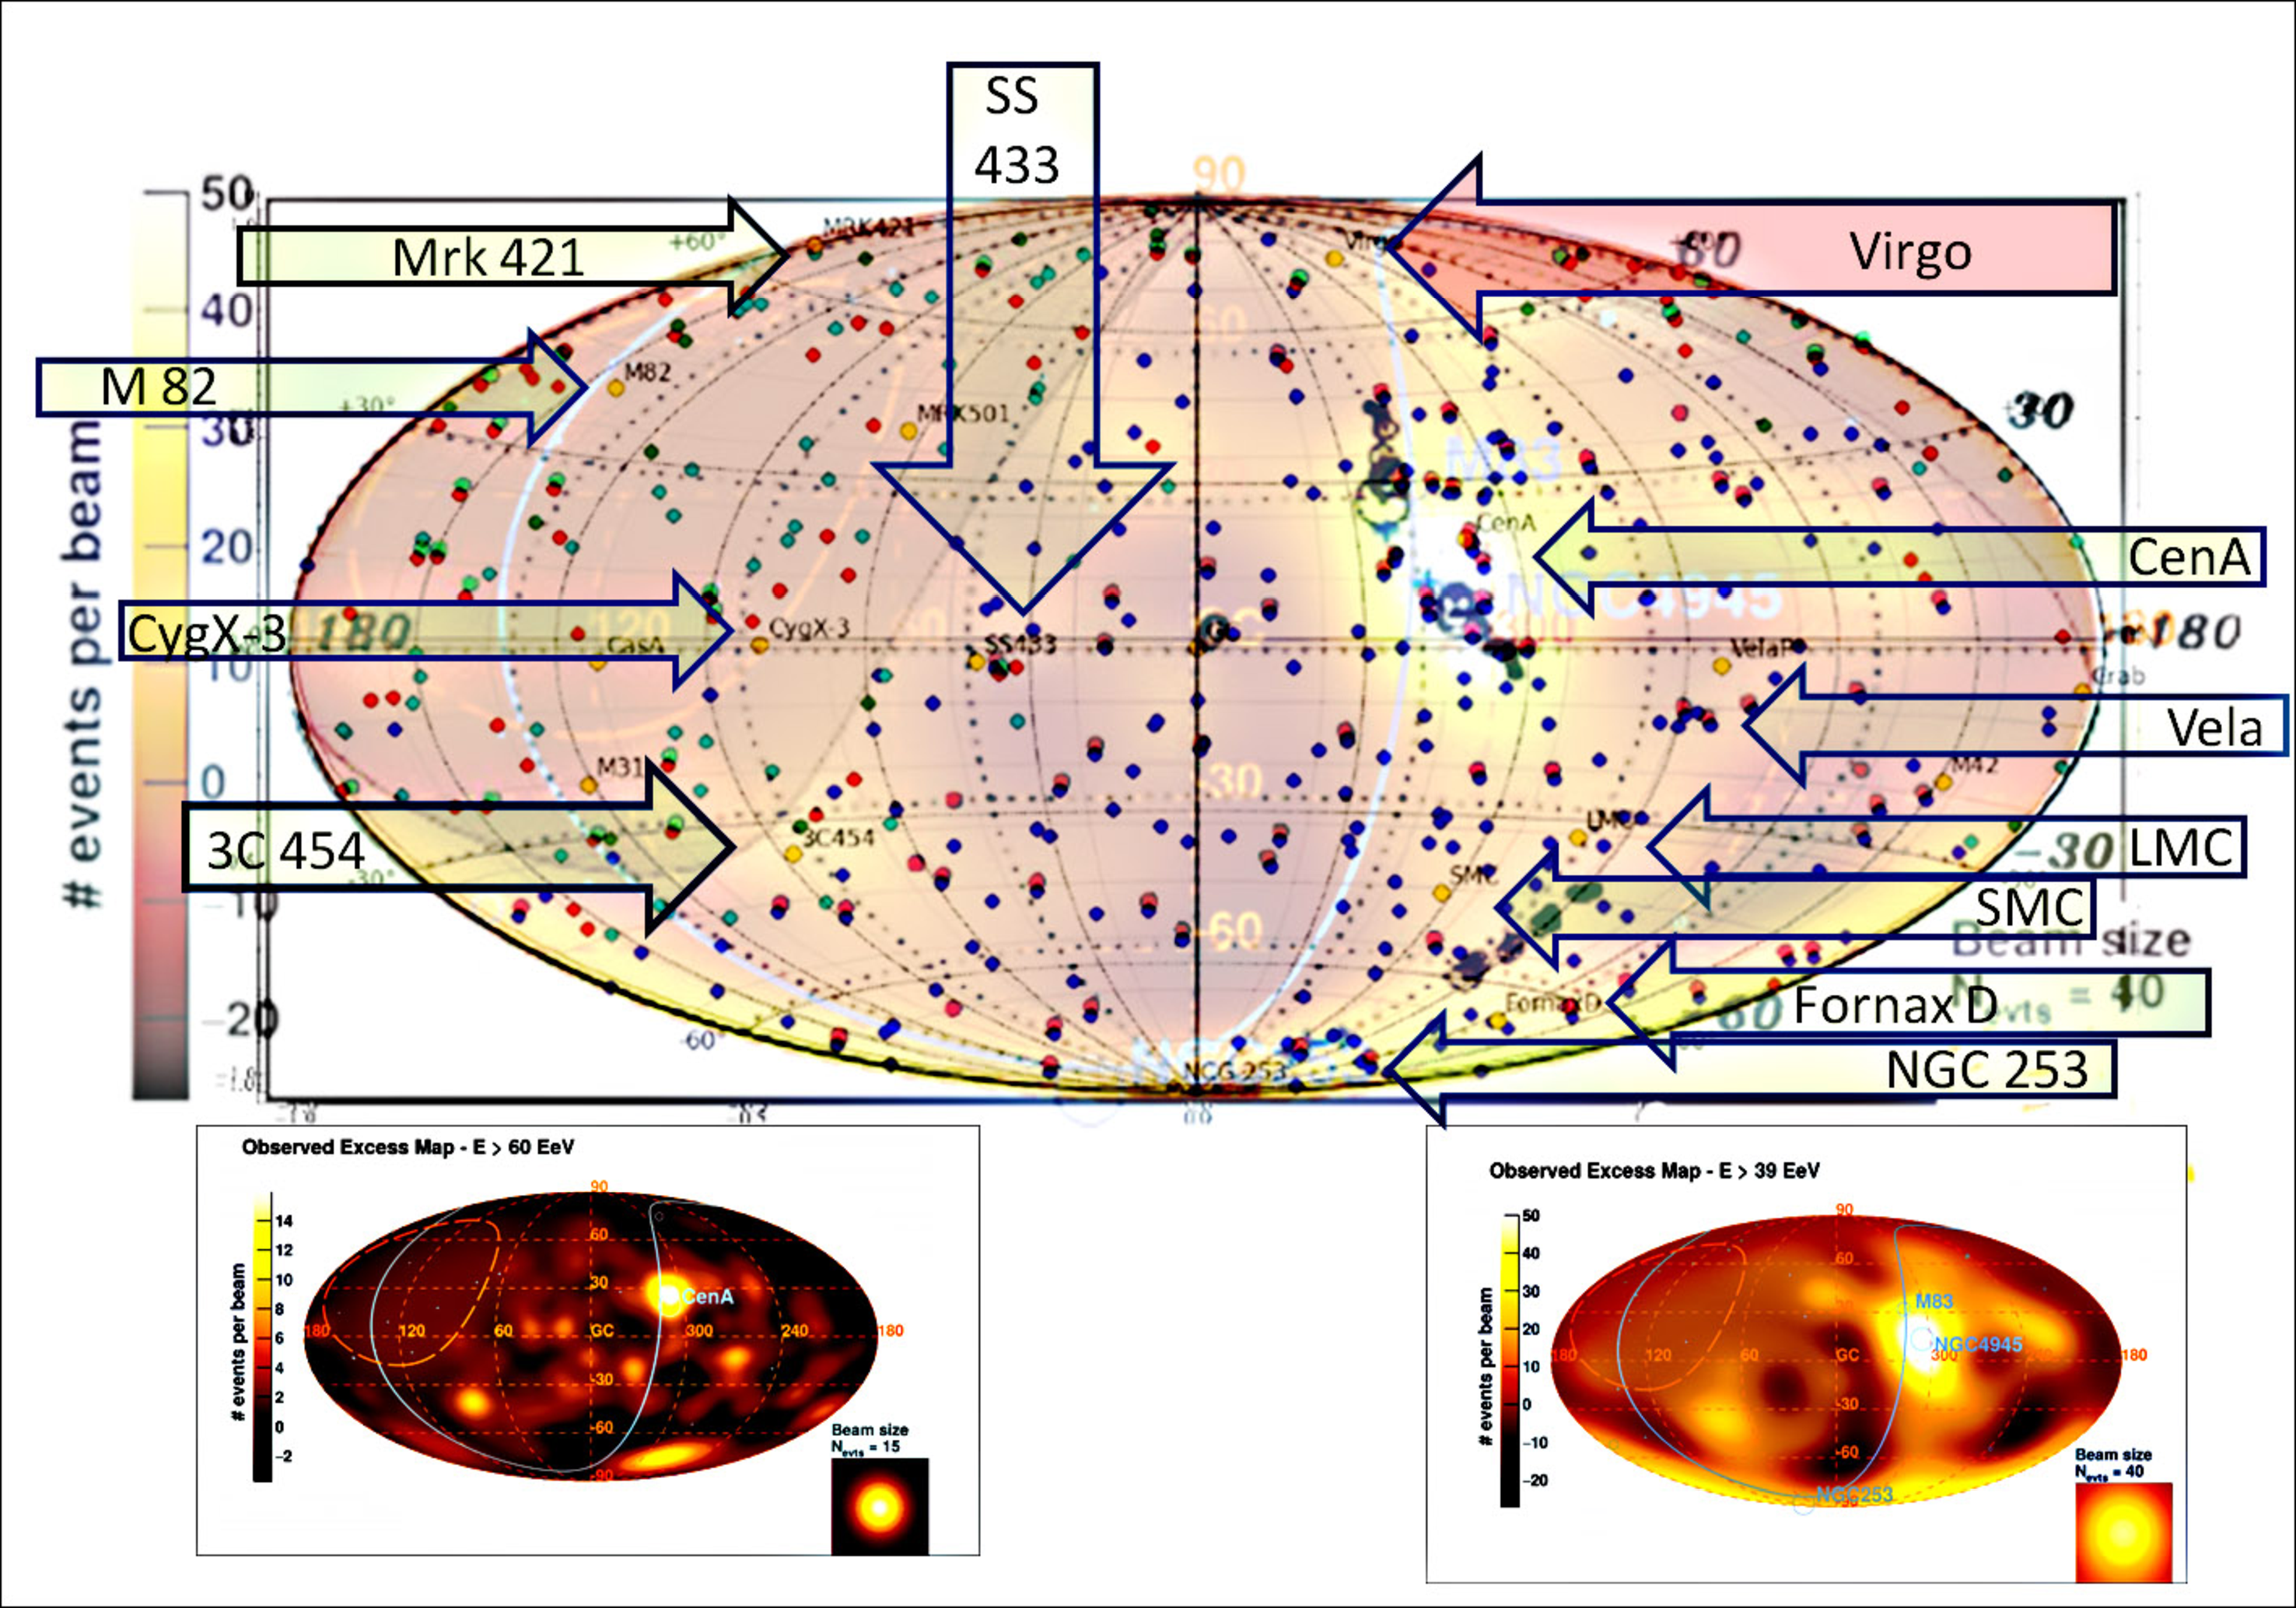
\includegraphics[width=0.5\linewidth]{data/uhecr-sources}
	\caption{Possible souces of \acrshort{uhecr} \cite{fargion2018ultra}}
	\label{fig:uhecr-sources}
\end{figure} \\
The spectrum of this cosmic radiation is shown in figure \ref{fig:cr_spectrum}.
\begin{figure}[ht!]
	\centering
	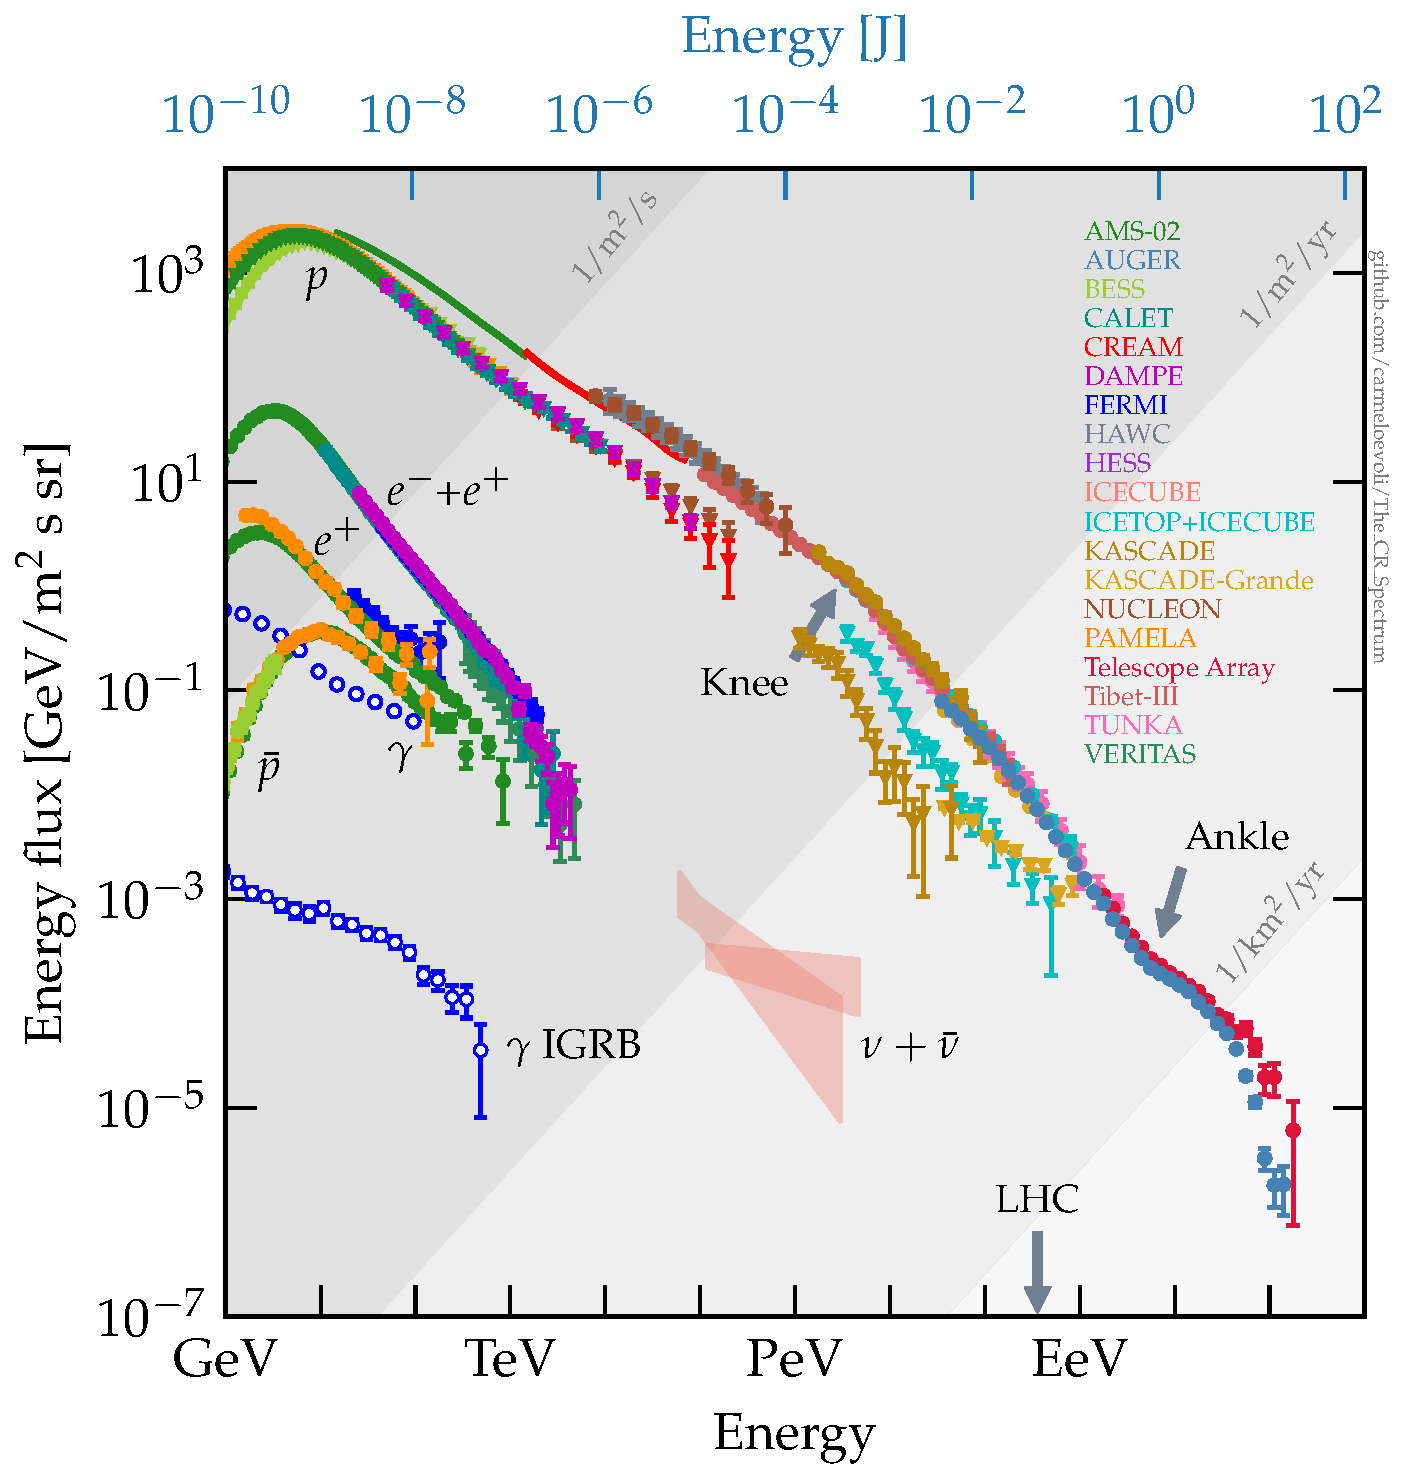
\includegraphics[width=0.75\linewidth]{data/cr_spectrum}
	\caption{Spectrum of cosmic radiation \cite{evoli_carmelo_2020_4396125}}
	\label{fig:cr_spectrum}
\end{figure} \\
There, measurements from different experiments are shown. The y axis shows the energy flux of cosmic rays in units of energy per second per square meter per solid angle $\frac{\text{GeV}}{\text{m}^2\cdot\text{s}\cdot\text{sr}}$. The x axis shows the primary energy of the cosmic rays, for comparison the upper axis shows the energy in units of Joule, the lower axis shows it in units of electron-Volt. Notable here is the much higher number of protons as compared to all other particles by two orders of magnitude. This allows one to make the reasonable assumption that most cosmic rays are protons or heavier nuclei. Energies above the labelled ankle originate almost exclusively from extragalactic sources.


One interesting observation is that the proton spectrum does not have a solid cutoff at $5\cdot10^{19}$\,eV of energy, rather it extends beyond it. This value is significant because it is calculated to be the \acrfull{gzkl}\cite{2021APh...12602526B}. This limit stems from high energy protons interacting with the microwave background radiation thus being lifted into an excited state which can decay through the interaction shown in equation \ref{eq:gzkl}.
\begin{equation}\label{eq:gzkl}
	\begin{aligned}
		\ce{\gamma + p &-> \Delta^+ &-> p + \pi^0} \\
		\ce{\gamma + p &-> \Delta^+ &-> n + \pi^+}
	\end{aligned}
\end{equation}
In both cases, the proton gets excited to a $\Delta^+$ resonance state, which can decay to a hadron and a pi meson. One possible decay product is a proton and a $\pi^0$, the other one a neutron and a $\pi^+$. Though this process, the proton loses roughly $20\,\%$ of its energy, since the energy prior to the interaction gets transferred to both resulting particles according to their relative masses. Should the proton then remain above the limit, the same interaction can take place again. It is unlikely that any proton at these energies can travel more than $100\,\cdot10^6\,\text{ly}$ without undergoing this interaction. Since most particles above the ankle in the proton specturm shown in figure \ref{fig:cr_spectrum} are of extragalactic origin, this means that virtually all protons with these high energies must have undergone this interaction, dropping them below the \acrshort{gzkl}.
The violation of this limit could be explained with a proposition by the Pierre Auger Observatory that most \acrshort{uhecr} are in fact heavier nuclei than single protons \cite{thepierreaugercollaboration2017inferences}.


The production mechanisms are not yet fully understood, though one possible mechanism involves active galaxy cores.
These are supermassive black holes at the centre of galaxies which feature an accretion disk. In the case of such a disk, a neutral particle can be on a decaying orbit which ends close to the Schwarzschild radius where they get ionised by the effective electric charge of the black hole which gets induced by the magnetic fields and spin of the black hole. The now positively charged particle gets accelerated to the highest energies and follows a spiral trajectory along the spin axis while the negative particle continues on the decaying trajectory.\cite{Tursunov_2020}
\begin{figure}[ht!]
	\centering
	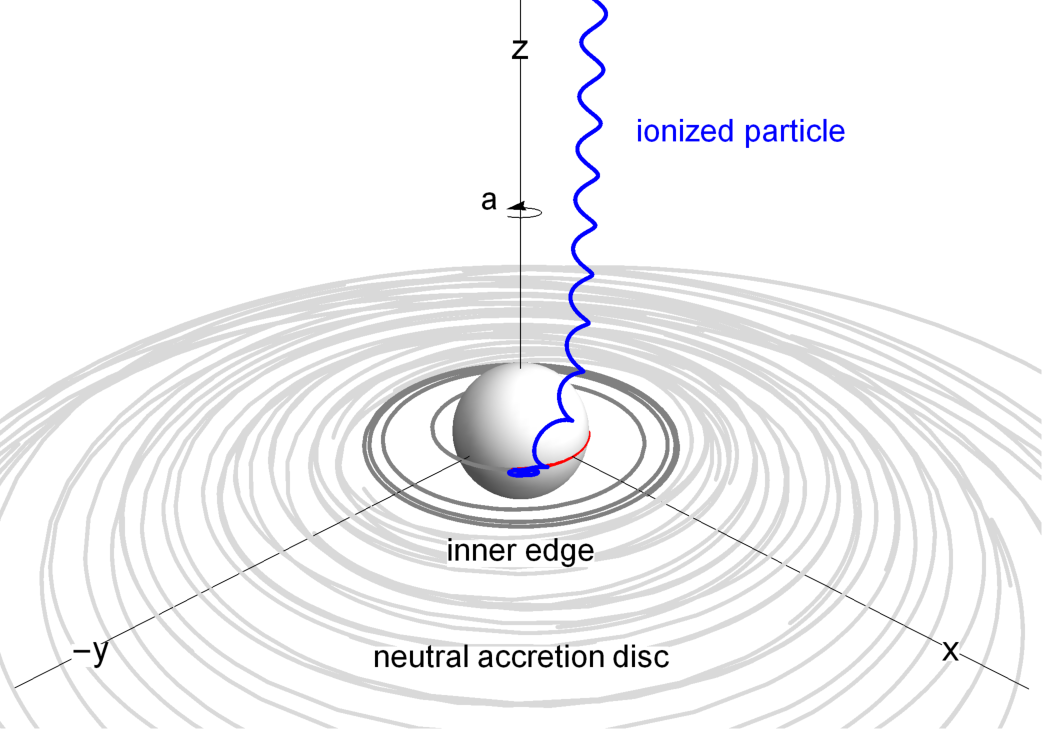
\includegraphics[width=0.5\linewidth]{data/uhecr-sm-bh}
	\caption{Trajectory of neutral particle around supermassive black hole \cite{Tursunov_2020}}
	\label{fig:uhecr-sm-bh}
\end{figure}\\
\clearpage
\subsection{Cosmic Air Showers}\label{subsec:airshowers}
When a cosmic ray hits the atmosphere, it interacts with the nucleons of the different molecules in air. Due to the relative abundance, it is most likely that the first interaction takes place between the primary particle and a Neutrogen nucleus. This interaction leaves nuclear fragments and $\pi$ mesons behind which can then interact with other air molecules again or - in the case of pions - decay. This creates a cascade of particles which continue along the trajectory towards the surface of earth. A picture of an air shower produced by a primary proton is shown in figure \ref{fig:proton-shower}. This image was created at the \acrfull{kit} with the simulation toolkit CORSIKA.
\begin{figure}[ht!]
	\centering
	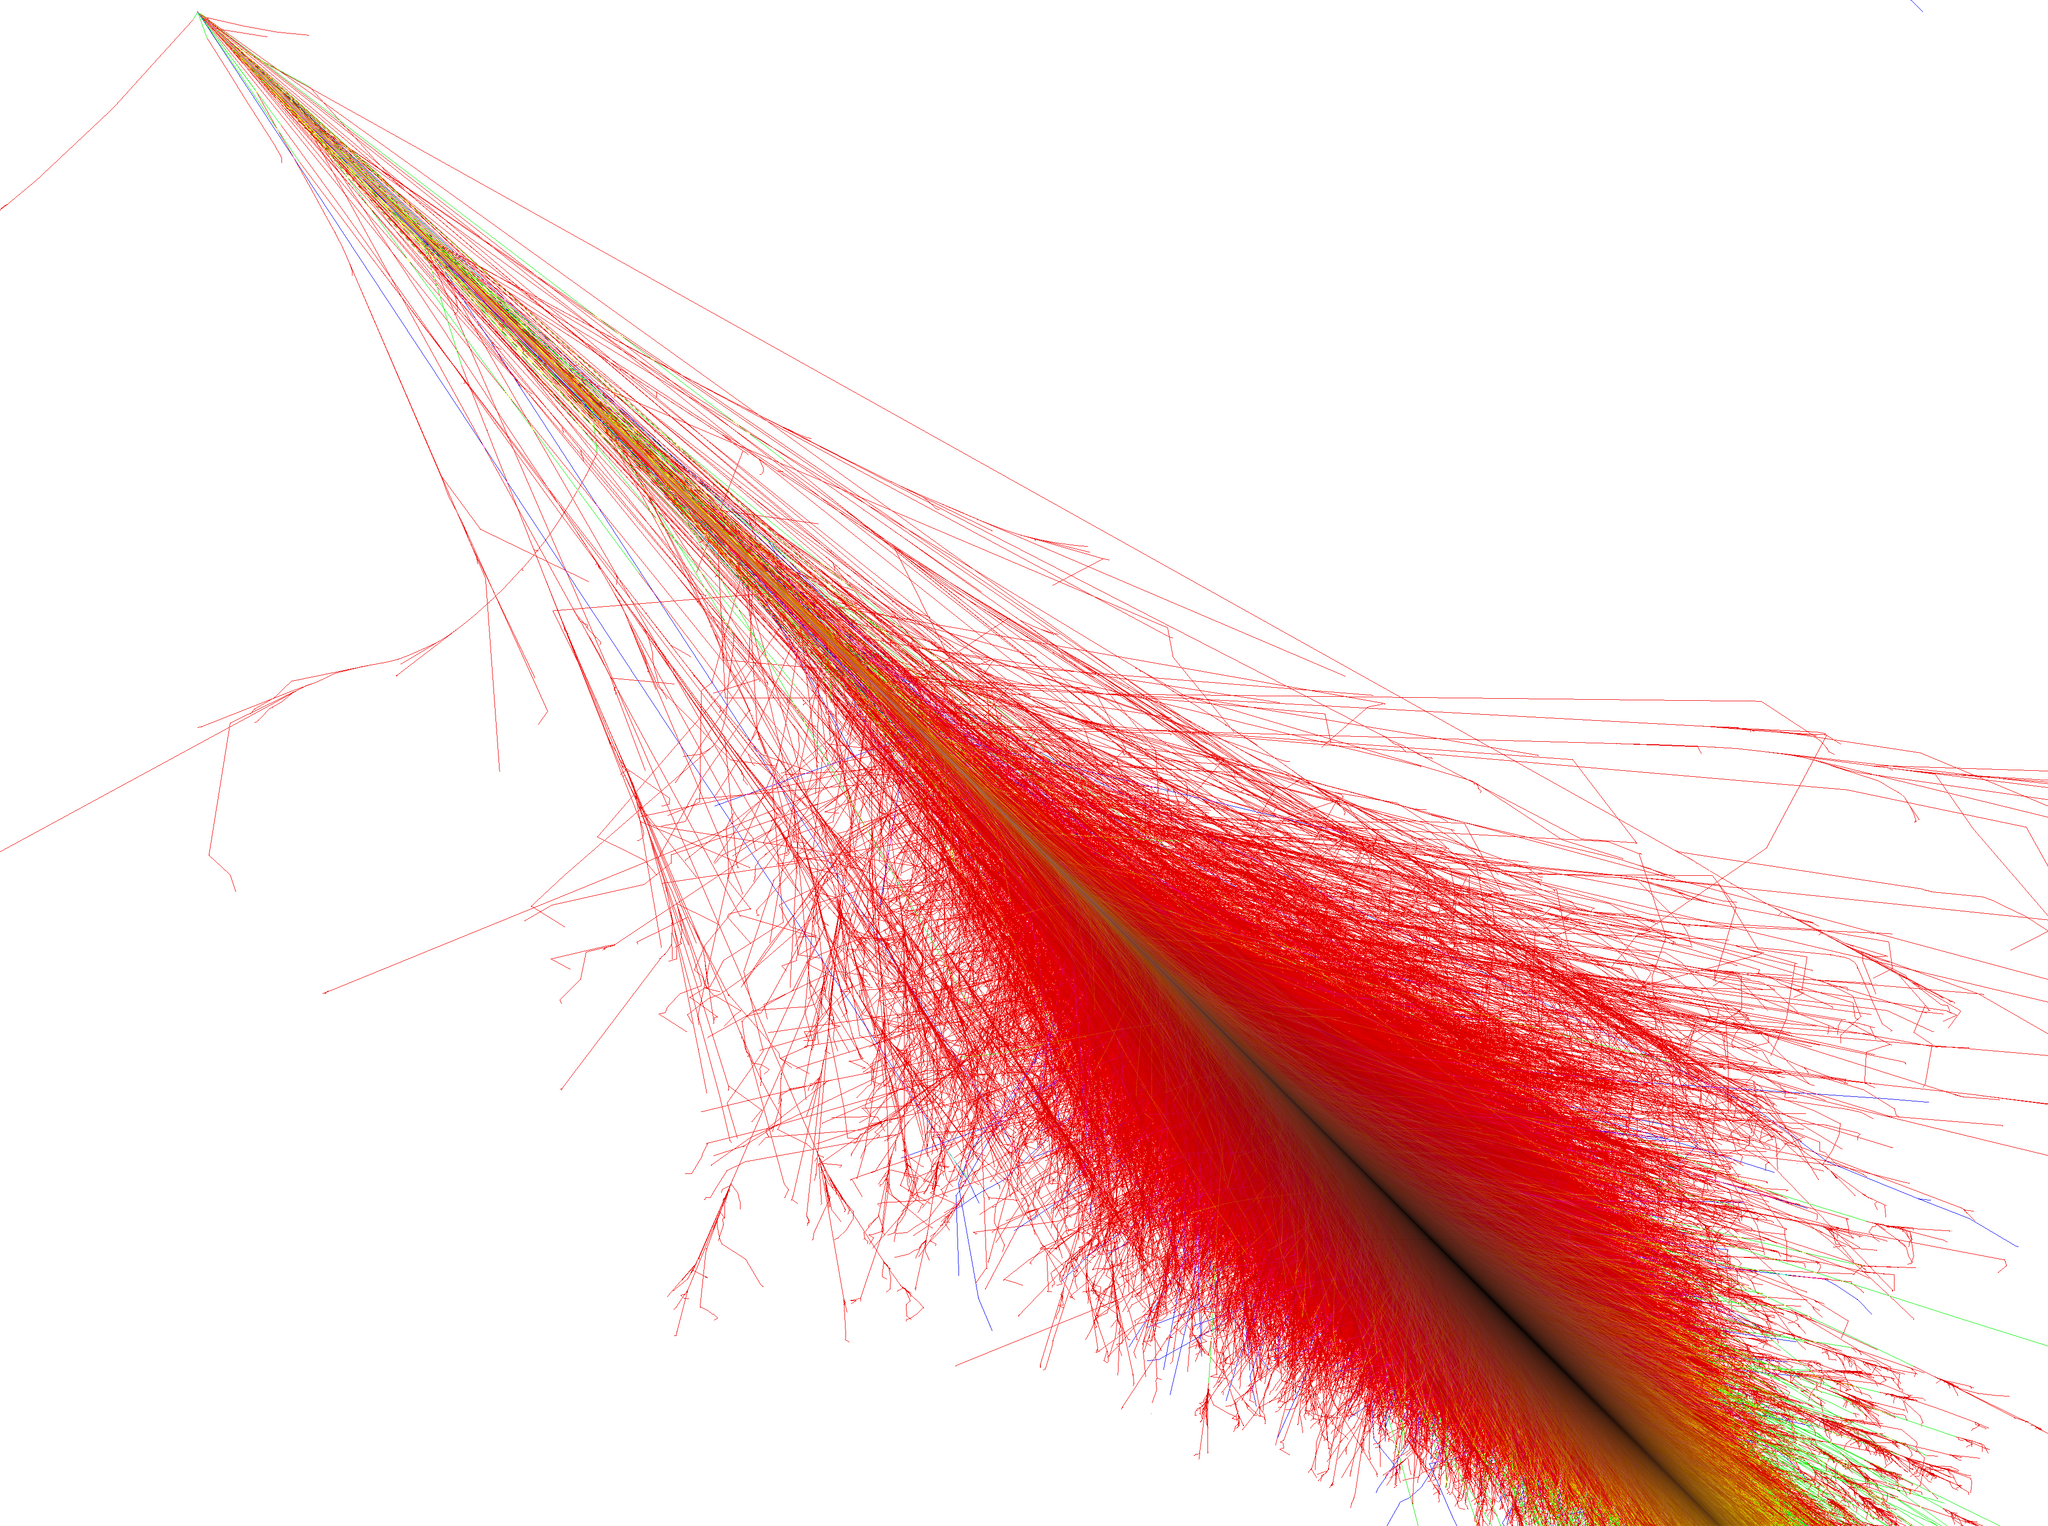
\includegraphics[width=0.8\linewidth]{data/shower-45}
	\caption{Proton Air Shower \cite{corsika-images}}
	\label{fig:proton-shower}
\end{figure} \\

The secondary particles can be divided into three different components, they are shown in figure \ref{fig:shower-components}.
Neutral Pions $\pi^0$ have two main decay modes. One is to two photons $\gamma$, the other to an electron positron pair and a photon. The probabilities decay cross section for the two gamma production is much higher than that of the $e^\pm + \gamma$ production though, with probabilities of roughly $98.823$ and $1.174\,\%$.\cite[1213]{10.1093/ptep/ptaa104} The other decay modes have orders of magnitude lower probabilities.
\begin{equation}
	\begin{aligned}
		\ce{\pi^0 &-> 2\gamma} \\
		\ce{\pi^0 &-> e^+ + e^- + \gamma} \\
	\end{aligned}
\end{equation}
The produced photons can then undergo pair production through which a lepton - anti lepton pair is produced. For this to occur, the photon needs to have an energy higher than twice the rest mass of the lepton. In the case of an electron positron pair, the rest energy is $511\,\text{keV}$ resulting in a minimum photon energy of $1022\,\text{keV}$. Any energy above this limit gets distributed evenly across both resulting particles as kinetic energy. In the \acrfull{com} system due to conservation of impulse, the pair travels in opposite directions to each other in a 90 degree angle to the original photon. In the laboratory system however, the resulting particles continue along the original trajectory with an angle between them.

Should the photon not have enough energy to produce a pair, it can be absorbed in an atom by raising the energy level of an electron in the shell or lose energy through Compton scattering.\\
In the case of a charged pion $\pi^\pm$, the by far most likely decay mode with a probability of $99.9877\,\%$ is to a muon $\mu^\pm$ and a muon-neutrino $\nu_\mu$.\cite[1211]{10.1093/ptep/ptaa104} The interaction is shown in equation \ref{eq:piondecay}.
\begin{equation}\label{eq:piondecay}
	\begin{aligned}
		\ce{\pi^+ &-> \mu^+ + \nu_\mu} \\
		\ce{\pi^- &-> \mu^- + \bar{\nu}_\mu}
	\end{aligned}
\end{equation}
\begin{figure}[ht!]
	\centering
	\begin{tikzpicture}
		\draw[->] (0,0.5) node[above] {primary particle} -- ++(0,-1.5) coordinate(primary);
		\draw[->] (primary) -- ++(-175:1.5) node[above] {$\pi^0$} -- ++(-175:2) coordinate (pi0);
		\draw[->] (primary) -- ++(-105:1) node[left] {$\pi^\pm$} -- ++(-105:1.5) coordinate (pipm);
		\draw[->] (primary) -- ++(-35:1) -- ++ (-35:2) coordinate (zn);
		
		\draw[->] (pi0) -- ++(-160:1) coordinate(gamma) node[above right] {$\gamma$};
		\draw[->] (pi0) -- ++(-130:1) node[below right] {$\gamma$};
		\draw[->] (gamma) -- ++(-165:1) node[above] {$e^\pm$};
		\draw[->] (gamma) -- ++(-155:1) node[below] {$e^\mp$};
		
		\draw[->] (pipm) -- ++(-110:1) node[left] {$\mu^\pm$};
		
		\draw[->] (zn) -- ++(-10:1) node[above] {p};
		\draw[->] (zn) -- ++(-30:1) node[below] {n};
		
		\draw[thin, dashed] (-2,0) -- ++(0,-5) ++ (-0.5,0) node[left] {Electromagnetic};
		\draw[thin, dashed] (2,0) -- ++(0,-5) ++(-1,0) node[left] {Muonic} ++(1.5,0) node[right] {Hadronic};
	\end{tikzpicture}
	\caption{Components of a cosmic air shower}
	\label{fig:shower-components}
\end{figure}
The figure does not show all interactions, nor does it show the Neutrinos produced through the different interactions.
The shower impact is dependent on the type of primary particle and its energy. In the case of \acrshort{uhecr}, the showers are classified as \acrfull{eas} which feature a larger footprint area and higher particle multiplicity on earth.

A different interaction of \acrshort{uhecr} with the atmosphere is the Cherenkov radiation. Due to the highly relativistic energies of the particles they travel faster than the local speed of light. In order to calculate the velocity of the particle, the relationship in Equation \ref{eq:lorentz-betagamma} can be used and solved for $\beta=\frac{v}{c_0}$.
\begin{equation} \label{eq:lorentz-betagamma}
	\beta\frac{1}{\sqrt{1 - \beta^2}} = \beta\gamma = \frac{E_{kin}}{E_{rest}}
\end{equation}
\begin{equation}
	\beta=\frac{1}{\sqrt{1 + \left(\frac{E_{rest}}{E_{kin}}\right)^2}}
\end{equation}

In the example of the Oh-My-God particle with an energy of $3.2\cdot10^{20}\,\text{eV}$ which is assumed to have been a proton with a rest energy of $\approx938.272\,\text{MeV}$, this calculates to
\begin{equation}
	\frac{E_{kin}}{E_{rest}} = \frac{3.2\cdot10^{20}\,\text{eV}}{938.27208816\,\text{MeV}}
\end{equation}
\begin{equation}
	\beta=\frac{1}{\sqrt{1 + 8.597212025587174\cdot10^{-24}}}\approx1.
\end{equation}
Given the refractive index of Air of $n\approx1.00028$ for visible light, the particle travels faster than the local speed of light. This causes light in the UV spectrum to be emitted comparable to a Mach cone in situations where an object travels faster than the speed of sound in a medium.
\begin{figure}[ht!]
	\centering
	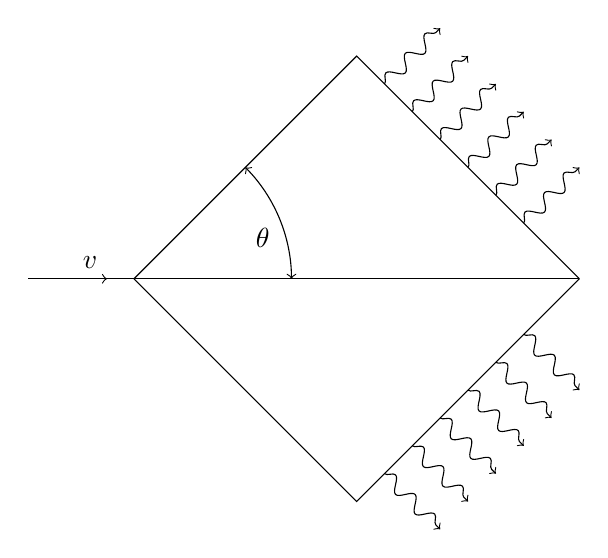
\begin{tikzpicture}
		\draw[->] (0,0) -- ++(1,0) node[above left] {$v$};
		\draw (0,0) -- ++(7,0) coordinate (tip);
		
		\draw (tip) -- ++(135:4) -- ++(-135:2) coordinate(top) -- ++(-135:2);
		\draw[->,decorate, decoration=snake] (tip) ++(135:1.0) -- ++(45:1);
		\draw[->,decorate, decoration=snake] (tip) ++(135:1.5) -- ++(45:1);
		\draw[->,decorate, decoration=snake] (tip) ++(135:2.0) -- ++(45:1);
		\draw[->,decorate, decoration=snake] (tip) ++(135:2.5) -- ++(45:1);
		\draw[->,decorate, decoration=snake] (tip) ++(135:3.0) -- ++(45:1);
		\draw[->,decorate, decoration=snake] (tip) ++(135:3.5) -- ++(45:1);
		
		\draw (tip) -- ++(-135:4) -- ++(135:4);
		\draw[->,decorate, decoration=snake] (tip) ++(-135:1.0) -- ++(-45:1);
		\draw[->,decorate, decoration=snake] (tip) ++(-135:1.5) -- ++(-45:1);
		\draw[->,decorate, decoration=snake] (tip) ++(-135:2.0) -- ++(-45:1);
		\draw[->,decorate, decoration=snake] (tip) ++(-135:2.5) -- ++(-45:1);
		\draw[->,decorate, decoration=snake] (tip) ++(-135:3.0) -- ++(-45:1);
		\draw[->,decorate, decoration=snake] (tip) ++(-135:3.5) -- ++(-45:1);
		
		\draw[<->] (top) arc(45:22.5:2) coordinate(theta) arc(22.5:0:2);
		\node[below left] at (theta) {$\theta$};
	\end{tikzpicture}
	\caption{Geometry of Cherenkov radiation.}
	\label{fig:cherenkov}
\end{figure}\\
The angle $\theta$ can be calculated through the relation $\cos\left(\theta\right)=\frac{1}{n\beta}$
\clearpage
\subsection{Detection methods}

The detection of \acrshort{uhecr} can be done through three main methods.\\
Two depend on the cosmic air showers described in the section \ref{subsec:airshowers}, namely the muonic and the electromagnetic component. The other method depends on the Cherenkov radiation where UV telescopes can be used to detect the UV light directly. By observing the same source through multiple locations, the origin can be reconstructed.
A popular example of a particle being detected through these means is the so called Oh-My-God particle, likely a proton or heavier nucleus with an energy of  $3.2\pm0.9\cdot10^{20}\,\text{eV}$ of energy. This particular particle is interesting since it was the first particle to exceed the \acrshort{gzkl}. It has been detected by the HiRes detector in Utah.

A method using the electromagnetic component of a cosmic air shower exploits the fact that the frequencies lie in the radio range\cite{NELLES201513} and can be detected through normal radio Antennae\cite{SCHRODER20171}. Due to the polarisation of the radio signal, often multiple antennae with different polarisation characteristics are used.

\begin{figure}[ht!]
	\centering
	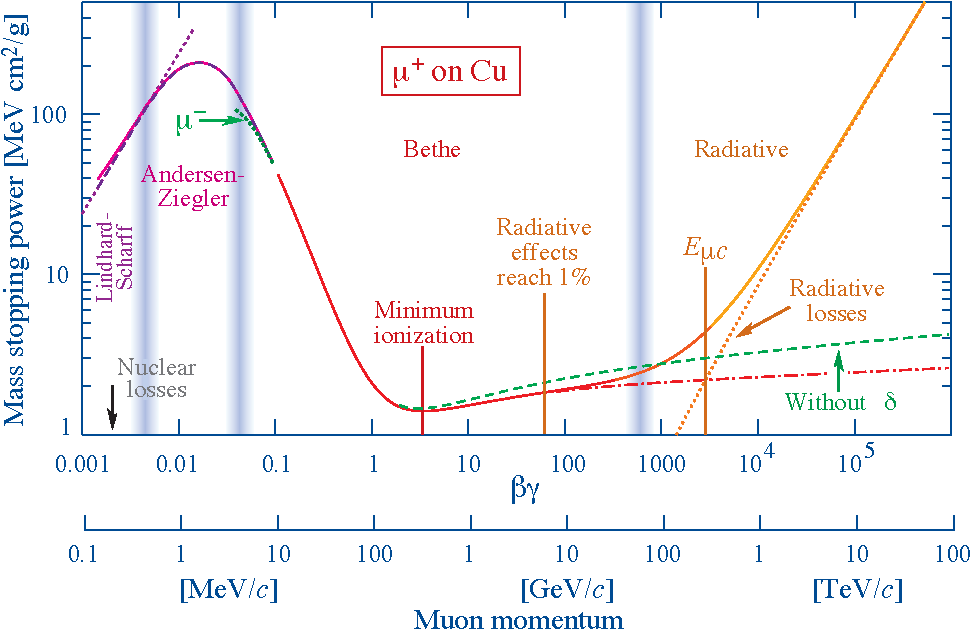
\includegraphics[width=\linewidth]{data/bethe-bloch}
	\caption{Expected energy deposit $\left\langle-\od{E}{x}\right\rangle$ of $\mu^+$ in copper \cite[536]{10.1093/ptep/ptaa104}}
	\label{fig:bethe-bloch}
\end{figure}
Another method is to detect the muonic component, this can be done through Scintillator detectors. Due to the muon being a charged particle, it interacts with matter and deposits energy according to figure \ref{fig:bethe-bloch}. The expected amount of deposited energy for a charged particle in matter can be described by the Bethe-Bloch formalism for $0.1\leq\beta\gamma\leq10^3$. Notable is that the deposited energy mainly depends on the relativistic speed of the particle described by $\beta\gamma$ where $\beta$ is the ratio of the velocity and speed of light and $\gamma$ the Lorentz factor. This is especially useful since it also equals the ratio between kinetic and rest energy. Figure \ref{fig:bethe-bloch} shows the mass stopping power of positive muons in copper with the Bethe-Bloch formalism describing the middle section.


Certain materials can give off this energy via photons, a process which is known as scintillation. Figure \ref{fig:scintillator} shows the mechanism through which scintillation occurs.
\begin{figure}[ht!]
	\centering
	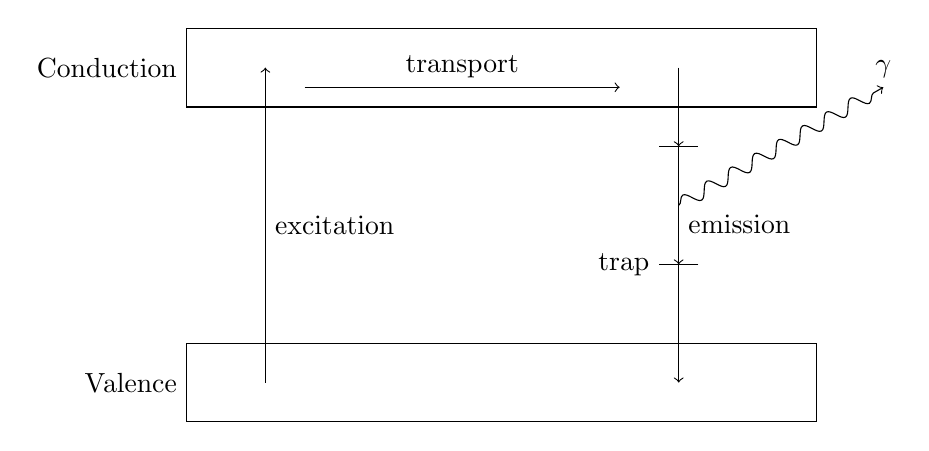
\begin{tikzpicture}[->]
		\draw (0,0) rectangle++(8,1);
		\draw (0,-3) rectangle++(8,-1);
		
		\draw (1,-3.5) -- ++(0,2) node[right] {excitation} -- ++(0,2);
		
		\draw (1.5,0.25) -- ++(2,0) node [above] {transport} -- ++(2,0);
		
		\draw[-] (6,-0.5) -- ++(0.5,0);
		\draw[-] (6.5,-2) -- ++(-0.5,0) node [left] {trap};
		
		\draw (6.25,0.5) -- ++(0,-1);
		\draw (6.25,-0.5) -- ++(0,-0.75) coordinate(emission) -- ++(0,-0.75);
		\draw (6.25,-2) -- ++(0,-1.5);
		
		\draw[decorate, decoration=snake] (emission) -- ++(30:3) node [above] {$\gamma$};
		\node[below right] at (emission) {emission};
		
		
		\node[left] at (0,0.5) {Conduction};
		\node[left] at (0,-3.5) {Valence};
	\end{tikzpicture}
	\caption{Mechanism for inorganic crystal scintillators}
	\label{fig:scintillator}
\end{figure}
First, an electron is excited from the valence band into the conduction band through energy deposit from an incident particle. This electron then is transported through the conduction band where it can drop back down to the valence band. Though if it dropped back directly, a photon would be emitted which could immediately excite another electron in the valence band. What makes scintillators special is the existence of traps which reduce the energy of the emitted photons. Those photons then do not have enough energy to excite electrons in the material so they can pass through it. With the use of a photomultiplier, the emitted photons can then be detected. One type of Photomultiplier is the \acrfull{sipm}, which is an array of single-photon avalanche diode which are photodiodes operating above the reverse-bias break-over voltage resulting in an avalanche upon interaction with even a single photon. The multiplicity of avalanches then is related to the number of photons interacting with the photomultiplier.

\section{Detectors}
\subsection{Station}
Each detector station consists of a Scintillator with \acrshort{sipm} assembly, a readout board and Raspberry Pi single-board computer and is called a \acrfull{cdu}.
\begin{figure}[H]
	\centering
	\begin{tikzpicture}
		\node [anchor=south west] at (0,0) {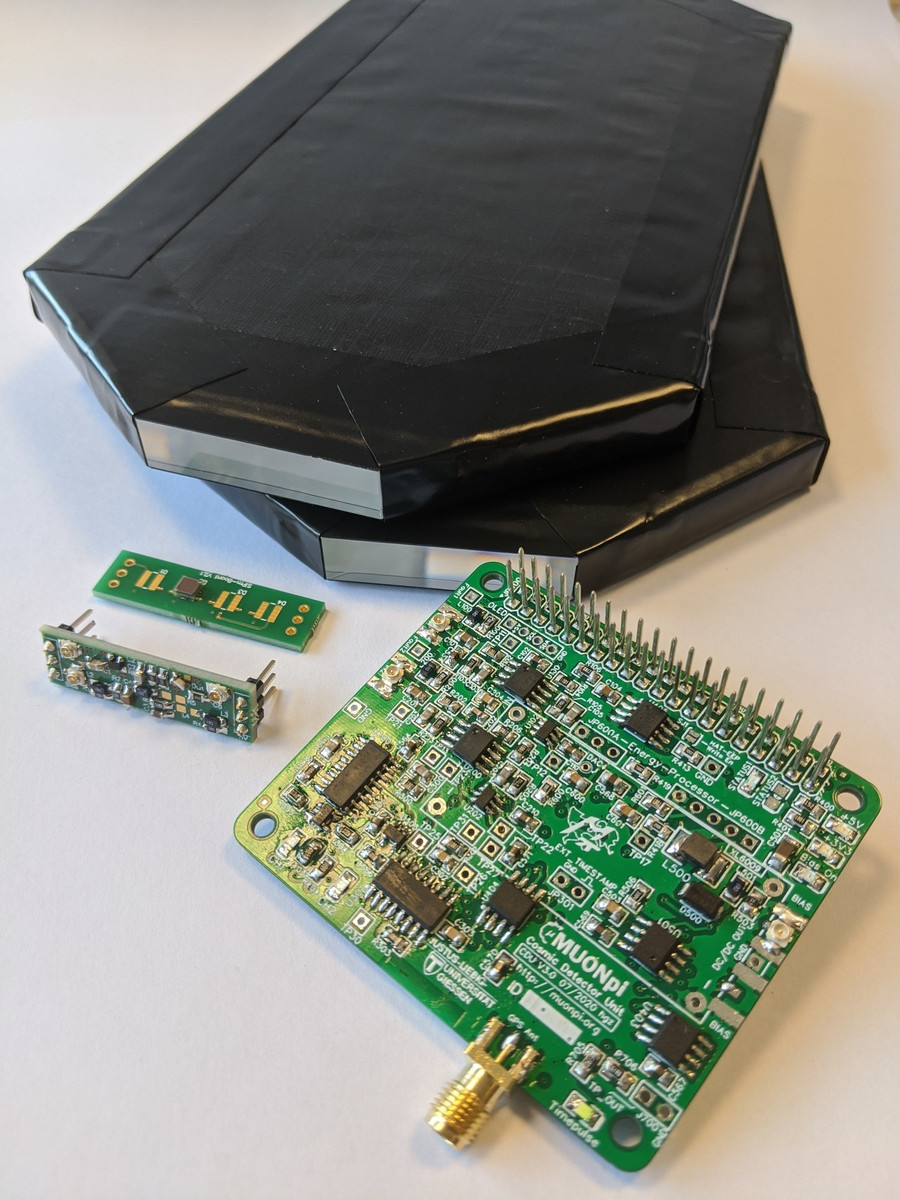
\includegraphics[width=0.4\linewidth]{data/station-assembly}};
		
		\draw[fill=black] (4,7) circle(0.1) -- ++(3,-1) node[below right] {Scintillator};
		\draw[fill=black] (1,4.5) circle(0.1) -- ++(-2,1) node[above left] {SiPM};
		\draw[fill=black] (0.75,3.5) circle(0.1) -- ++(-2,0) node[left] {Preamplifier};
		\draw[fill=black] (4,3) circle(0.1) -- ++(3,0) node[right] {Readout board};
	\end{tikzpicture}
	\caption{Detector station assembly without Raspberry Pi computer}
	\label{fig:station_assembly}
\end{figure}
In figure \ref{fig:station_assembly} each component excluding the Raspberry Pi is shown. The SiPM is still detached from the Scintillator for this picture since it would not be visible as separate part otherwise. The preamplifier is part of the SiPM assembly and prepares the signal to the readout board in order to prevent loss of signal over the transmission line. The readout board supports two input channels which can be linked logically either per AND or XOR, though per default only one channel is used.

The readout board uses a ublox NEO GNSS receiver chip which features an interrupt input to accurately timestamp input signals with a maximum resolution of $21\,\text{ns}$ \cite{ublox-datasheet} with a deadtime of $100\,\text{ms}$.
This deadtime makes it unsuitable for high frequency applications though due to the scintillator size of $286.5\,\text{cm}^2$ and an integral intensity of Muons over the whole energy spectrum above $1\,\text{GeV}$ of $1\,\text{cm}^{-2}\text{min}^{-1}$\cite[512]{10.1093/ptep/ptaa104} the expected maximum detection rate of $4.7\,\text{Hz}$ is within the capabilities of this setup. \\
\clearpage
The detector software collects various information in addition to the timestamp with each event and sends it to the server via the \acrfull{mqtt} protocol. This is a text-based protocol providing reliable information transfer with minimal overhead\cite{mqtt}. Additional to the event information the station sends log information in regular intervals indicative of the current state of the detector station.
\subsection{Data exchange format}
\paragraph{Event messages} contain information about the event with additional details about the current state of the detector station. Each message consists of $8$ fields, one of which is part of the \acrshort{mqtt} message topic and $7$ are part of the payload. An example is shown in listing \ref{lst:mqtt-event}, the fields are described in table \ref{tab:event-message}.
\begin{lstfloat}[H]
	\centering
	\begin{verbatim}
		jlu/HBR16Lab105_1 1625745406.606430870 1625745406.606431974 26 13526 1 2 1
	\end{verbatim}
	\caption{Event message format example}
	\label{lst:mqtt-event}
\end{lstfloat}
\begin{table}[H]
	\centering
	\begin{tabular}{| c | c |}
		\hline
		\textbf{Position} & \textbf{Description} \\
		\hline
		$1$ & detector station user and id \\
		\hline
		$2$ & Nanosecond rising edge timestamp \\
		\hline
		$3$ & Nanosecond falling edge timestamp \\
		\hline
		$4$ & Time Accuracy in Nanoseconds \\
		\hline
		$5$ & $16$ bit event counter value from the detector station \\
		\hline
		$6$ & Bitflag for valid GNSS fix \\
		\hline
		$7$ & UTC Time flag \\
		\hline
		$8$ & GNSS time grid flag \\
		\hline
	\end{tabular}
	\caption{Event message field description}
	\label{tab:event-message}
\end{table}


\paragraph{Log messages} contain various information about the current station state and are formatted as shown in Listing \ref{lst:mqtt-log}, the unit field is not present in all log messages. A small excerpt of various log message identifiers is shown in Table \ref{tab:station_logs}.
\begin{lstfloat}[H]
	\centering
	\begin{verbatim}
		jlu/HBR16Lab105_1 <message identifier> <value> [unit]
	\end{verbatim}
	\caption{Log message format}
	\label{lst:mqtt-log}
\end{lstfloat}
\begin{table}[H]
	\centering
	\begin{tabular}{| c | c |}
		\hline
		\textbf{Identifier} & \textbf{Description} \\
		\hline
		\verb*|geoLongitude| & Longitude of the detector station \\
		\hline
		\verb*|geoLatitude| & Latitude of the detector station \\
		\hline
		\verb*|geoHeightMSL| & Vertical height above the reference ellipsoid surface \\
		\hline
		\verb*|geoHorAccuracy| & Horizontal accuracy of the GNSS signal \\
		\hline
		\verb*|geoVertAccuracy| & Vertical accuracy of the GNSS signal \\
		\hline
		\verb*|positionDOP| & Positional dilution of precision\footnotemark \\
		\hline
		\verb*|clockDrift| & Current inherent drift of the internal clock\\
		\hline
		\verb*|timeAccuracy| & Accuracy of the time measurement \\
		\hline
		\verb*|timeDOP| & Time dilution of precision \\
		\hline
	\end{tabular}
	\caption{Excerpt from detector station log message content}
	\label{tab:station_logs}
\end{table}
\footnotetext{\acrfull{dop}: Numerical value for the statistical dispersion of GNSS measurements}
Since the detector network is not at known locations but distributed across multiple cities and countries at different users locations, in order to be able to make attempts at particle reconstruction, the location information is one of the more important information from the log messages. Additionally to this, the accuracy measurement values are used to determine in what state the detector station is to be able to judge the data integrity.
\clearpage
\subsection{Network}
All detector stations are part of a larger network of detectors with a central data processor which analyses all incoming event data for possible coincidences. The entire analysis stack is shown in Figure \ref{fig:network-stack}.
\begin{figure}[H]
	\centering
	\begin{tikzpicture}[>=latex, ->]
		\node (scintillator) [draw, process, minimum height=1cm, minimum width=5cm] {Scintillator};
		\node (cdu) [below=of scintillator, draw, process, minimum height=1cm, minimum width=5cm] {Readout board};
		\node (raspi) [below=of cdu, draw, process, minimum height=1cm, minimum width=5cm] {Raspberry Pi};
		
		\node (mqtt) [right=of raspi, draw, process, minimum height=1cm] {MQTT};
		
		\node (server) [right=of mqtt, draw, process, minimum height=1cm, minimum width=5cm] {Server};
		\node (dnp) [above=of server, draw, process, minimum height=1cm, minimum width=5cm] {Network Processor};
		\node (db) [above=of dnp, draw, process, minimum height=1cm, minimum width=5cm] {Database};
		\node (analysis) [above=of db, draw, process, minimum height=1cm, minimum width=5cm] {Further analysis};
		
		\node (shower) [above=of scintillator] {Shower};
		
		\draw (shower) -- (scintillator) node [midway, right] {$\mu$};
		\draw (scintillator) -- (cdu);
		\draw (cdu) -- (raspi);
		\draw (raspi) -- (mqtt);
		\draw (mqtt) -- (server);
		\draw (server) -- (dnp);
		\draw (dnp) -- (db);
		\draw (db) -- (analysis);
	\end{tikzpicture}
	\caption{Detector network analysis stack}
	\label{fig:network-stack}
\end{figure}
A current overview of active and future stations in Europe can be seen in figure \ref{fig:station-overview}, additional stations are located in north America and Australia. 
\begin{figure}[H]
	\centering
	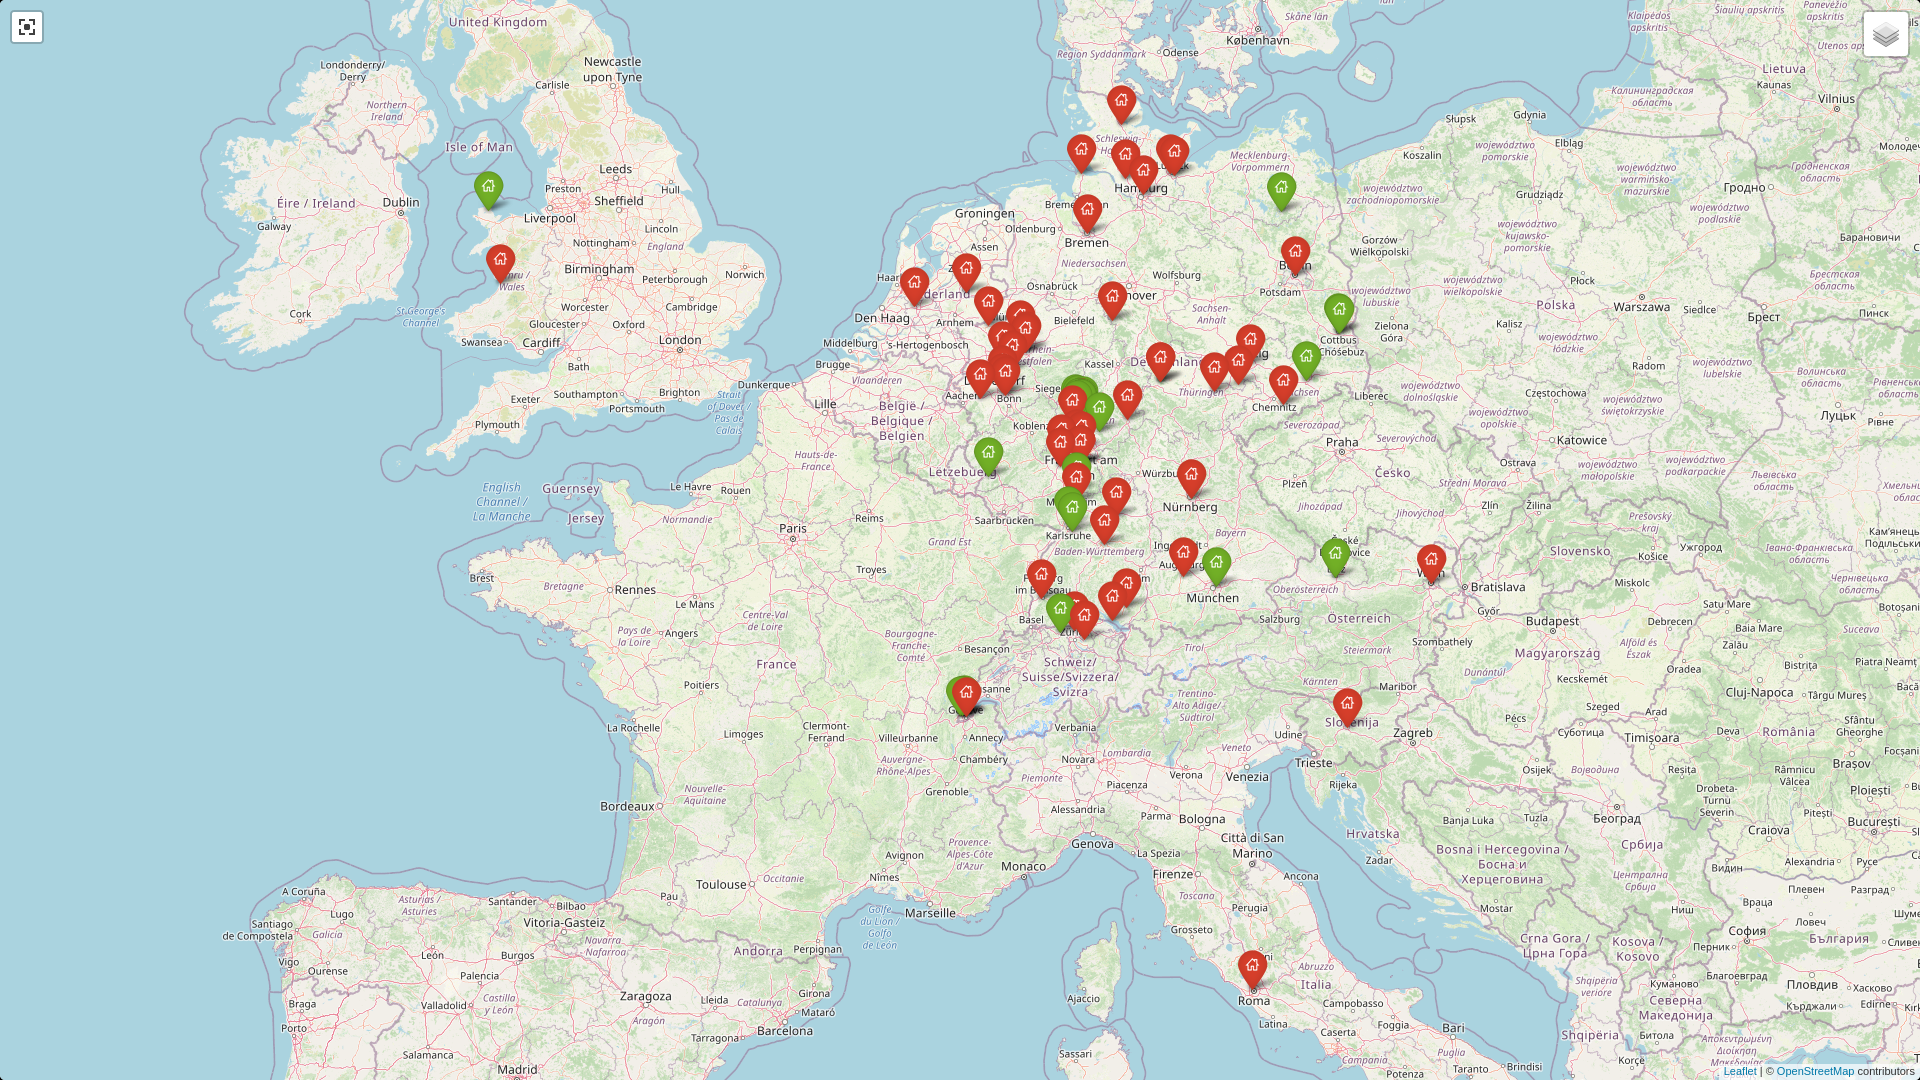
\includegraphics[width=0.7\linewidth]{data/detector-stations}
	\caption[Current overview of detector stations]{Current overview of detector stations\cite{muonpi}.\\Red: future stations\\Green: active stations}
	\label{fig:station-overview}
\end{figure}

\subsection{Data}
The shower front shape of a cosmic shower can initially be assumed to be a thick spherical cap with a thickness of $1\,\text{to}\,2\,\text{m}$\cite{grapes-3-2019}. This shape however fluctuates between shower events and measurements range from spherical cap shapes\cite{chitnis-2002} to conical shapes\cite{grapes-3-2019}. The thickness and deviation from the shape of a spherical cap introduce uncertainties in the calculations presented in this thesis in section \ref{sec:reconstruction}.
\begin{figure}[H]
	\centering
	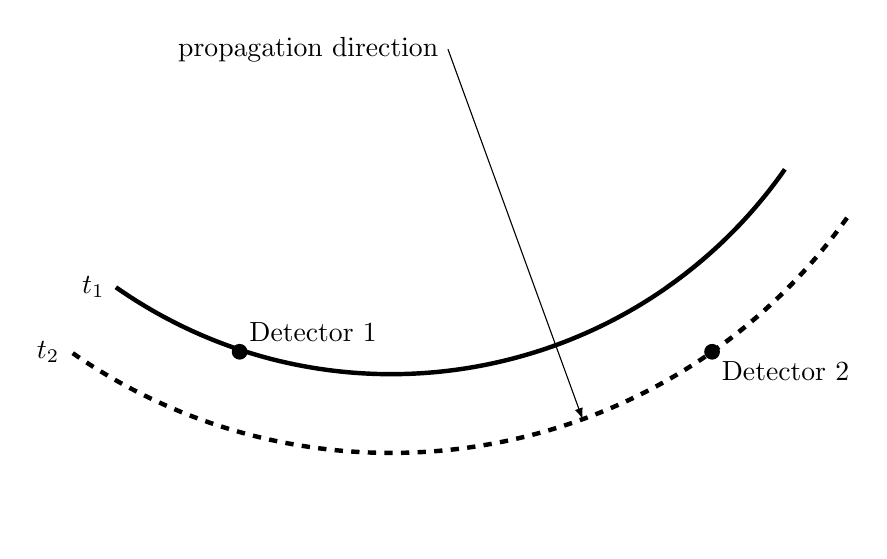
\begin{tikzpicture}
		\fill (0,0) coordinate(det1) circle(0.1) node[above right] {Detector 1};
		\fill (6,0) coordinate(det2) circle(0.1) node[below right] {Detector 2};
		\draw[ultra thick] (det2) ++ (125:1) arc(-55:-35:6.1) arc(-35:-125:6.1) node[left] {$t_1$};
		\draw[ultra thick, dashed] (det2) arc(-55:-35:7.1) arc(-35:-125:7.1) node[left] {$t_2$};
		\path (det2) arc(-55:-70:7.1) coordinate(source);
		\draw[<-, >=latex] (source) -- ++ (110:5) node[left] {propagation direction};
	\end{tikzpicture}
	\caption{Propagation of the shower front}
	\label{fig:data-shape}
\end{figure}
Figure \ref{fig:data-shape} shows the propagation of the shower front in relation to two detectors. Assuming both detectors have a detection efficiency of $100\,\%$, both will show an event at their respective timestamps $t_1$ and $t_2$. The time difference between both measured timestamps can help to reconstruct the direction of propagation, a method how to do this is shown later in this thesis.

Comparing the timestamps of single detector hits can be used to correlate single data points and combine them to coincidences.
\begin{figure}[H]
	\centering
	\begin{subfigure}{\linewidth}
		\caption{Short detector distance}
		\label{fig:histogram-data:close}
		\begin{tikzpicture}
			\begin{axis}[area style, xlabel={$\Delta{t}\,[\text{ns}]$},ylabel={$n$}, xmin=-600,xmax=600,width=\linewidth,height=0.2\textheight]% coordinates
				\addplot+[ybar interval,mark=no] table {data/jluHBR16Lab105_1_jluHBR16Lab105_DoublePaddle.hist};
			\end{axis}
		\end{tikzpicture}
	\end{subfigure}
	\begin{subfigure}{\linewidth}
		\caption{Medium detector distance}
		\label{fig:histogram-data:mid}
		\begin{tikzpicture}
			\begin{axis}[area style, xlabel={$\Delta{t}\,[\text{ns}]$},ylabel={$n$}, xmin=-600,xmax=600,width=\linewidth,height=0.2\textheight]]% coordinates
				\addplot+[ybar interval,mark=no] table {data/CERN1_CERN3.hist};
			\end{axis}
		\end{tikzpicture}
	\end{subfigure}
	\begin{subfigure}{\linewidth}
		\caption{Large detector distance}
		\label{fig:histogram-data:far}
		\begin{tikzpicture}
			\begin{axis}[area style, xlabel={$\Delta{t}\,[\text{ns}]$},ylabel={$n$}, xmin=-100000,xmax=100000,width=\linewidth,height=0.2\textheight]]% coordinates
				\addplot+[ybar interval,mark=no] table {data/simonglm0_mw1cfn0.hist};
			\end{axis}
		\end{tikzpicture}
	\end{subfigure}
	\caption{Coincidence time histograms for various distances}
	\label{fig:histogram-data}
\end{figure}
When recording all coincidence times of one detector pair the different times can be plotted in a histogram. Figure \ref{fig:histogram-data} shows histograms for three different detector pairs with different distances. The plot \ref{fig:histogram-data:close} shows the closest distance of a few meters, plot \ref{fig:histogram-data:mid} a medium distance of roughly $130\,\text{m}$ and plot \ref{fig:histogram-data:far} a distance of $950\,\text{km}$.

The closest distance shows the clearest signal and largest signal-to-noise ratio. However due to the location of both detectors, the GNSS signal is often weak which leads to a broad distribution due to low time resolution.

In the medium distance plot, a still significant signal is visible, though the signal-to-noise ratio is much lower. The lower number of entries is due to the shorter total runtime of this particular detector pair.

The furthest distance plot shows no significant signal over the random background.

This highlights the relationship between coincidence rate and detector distance as shown in figure \ref{fig:pair-count-rate}. There, a number of experiments have been performed in order to determine the coincidence rates for different distances. A linear fit has been applied to the experimental data.
\begin{figure}[H]
	\centering
	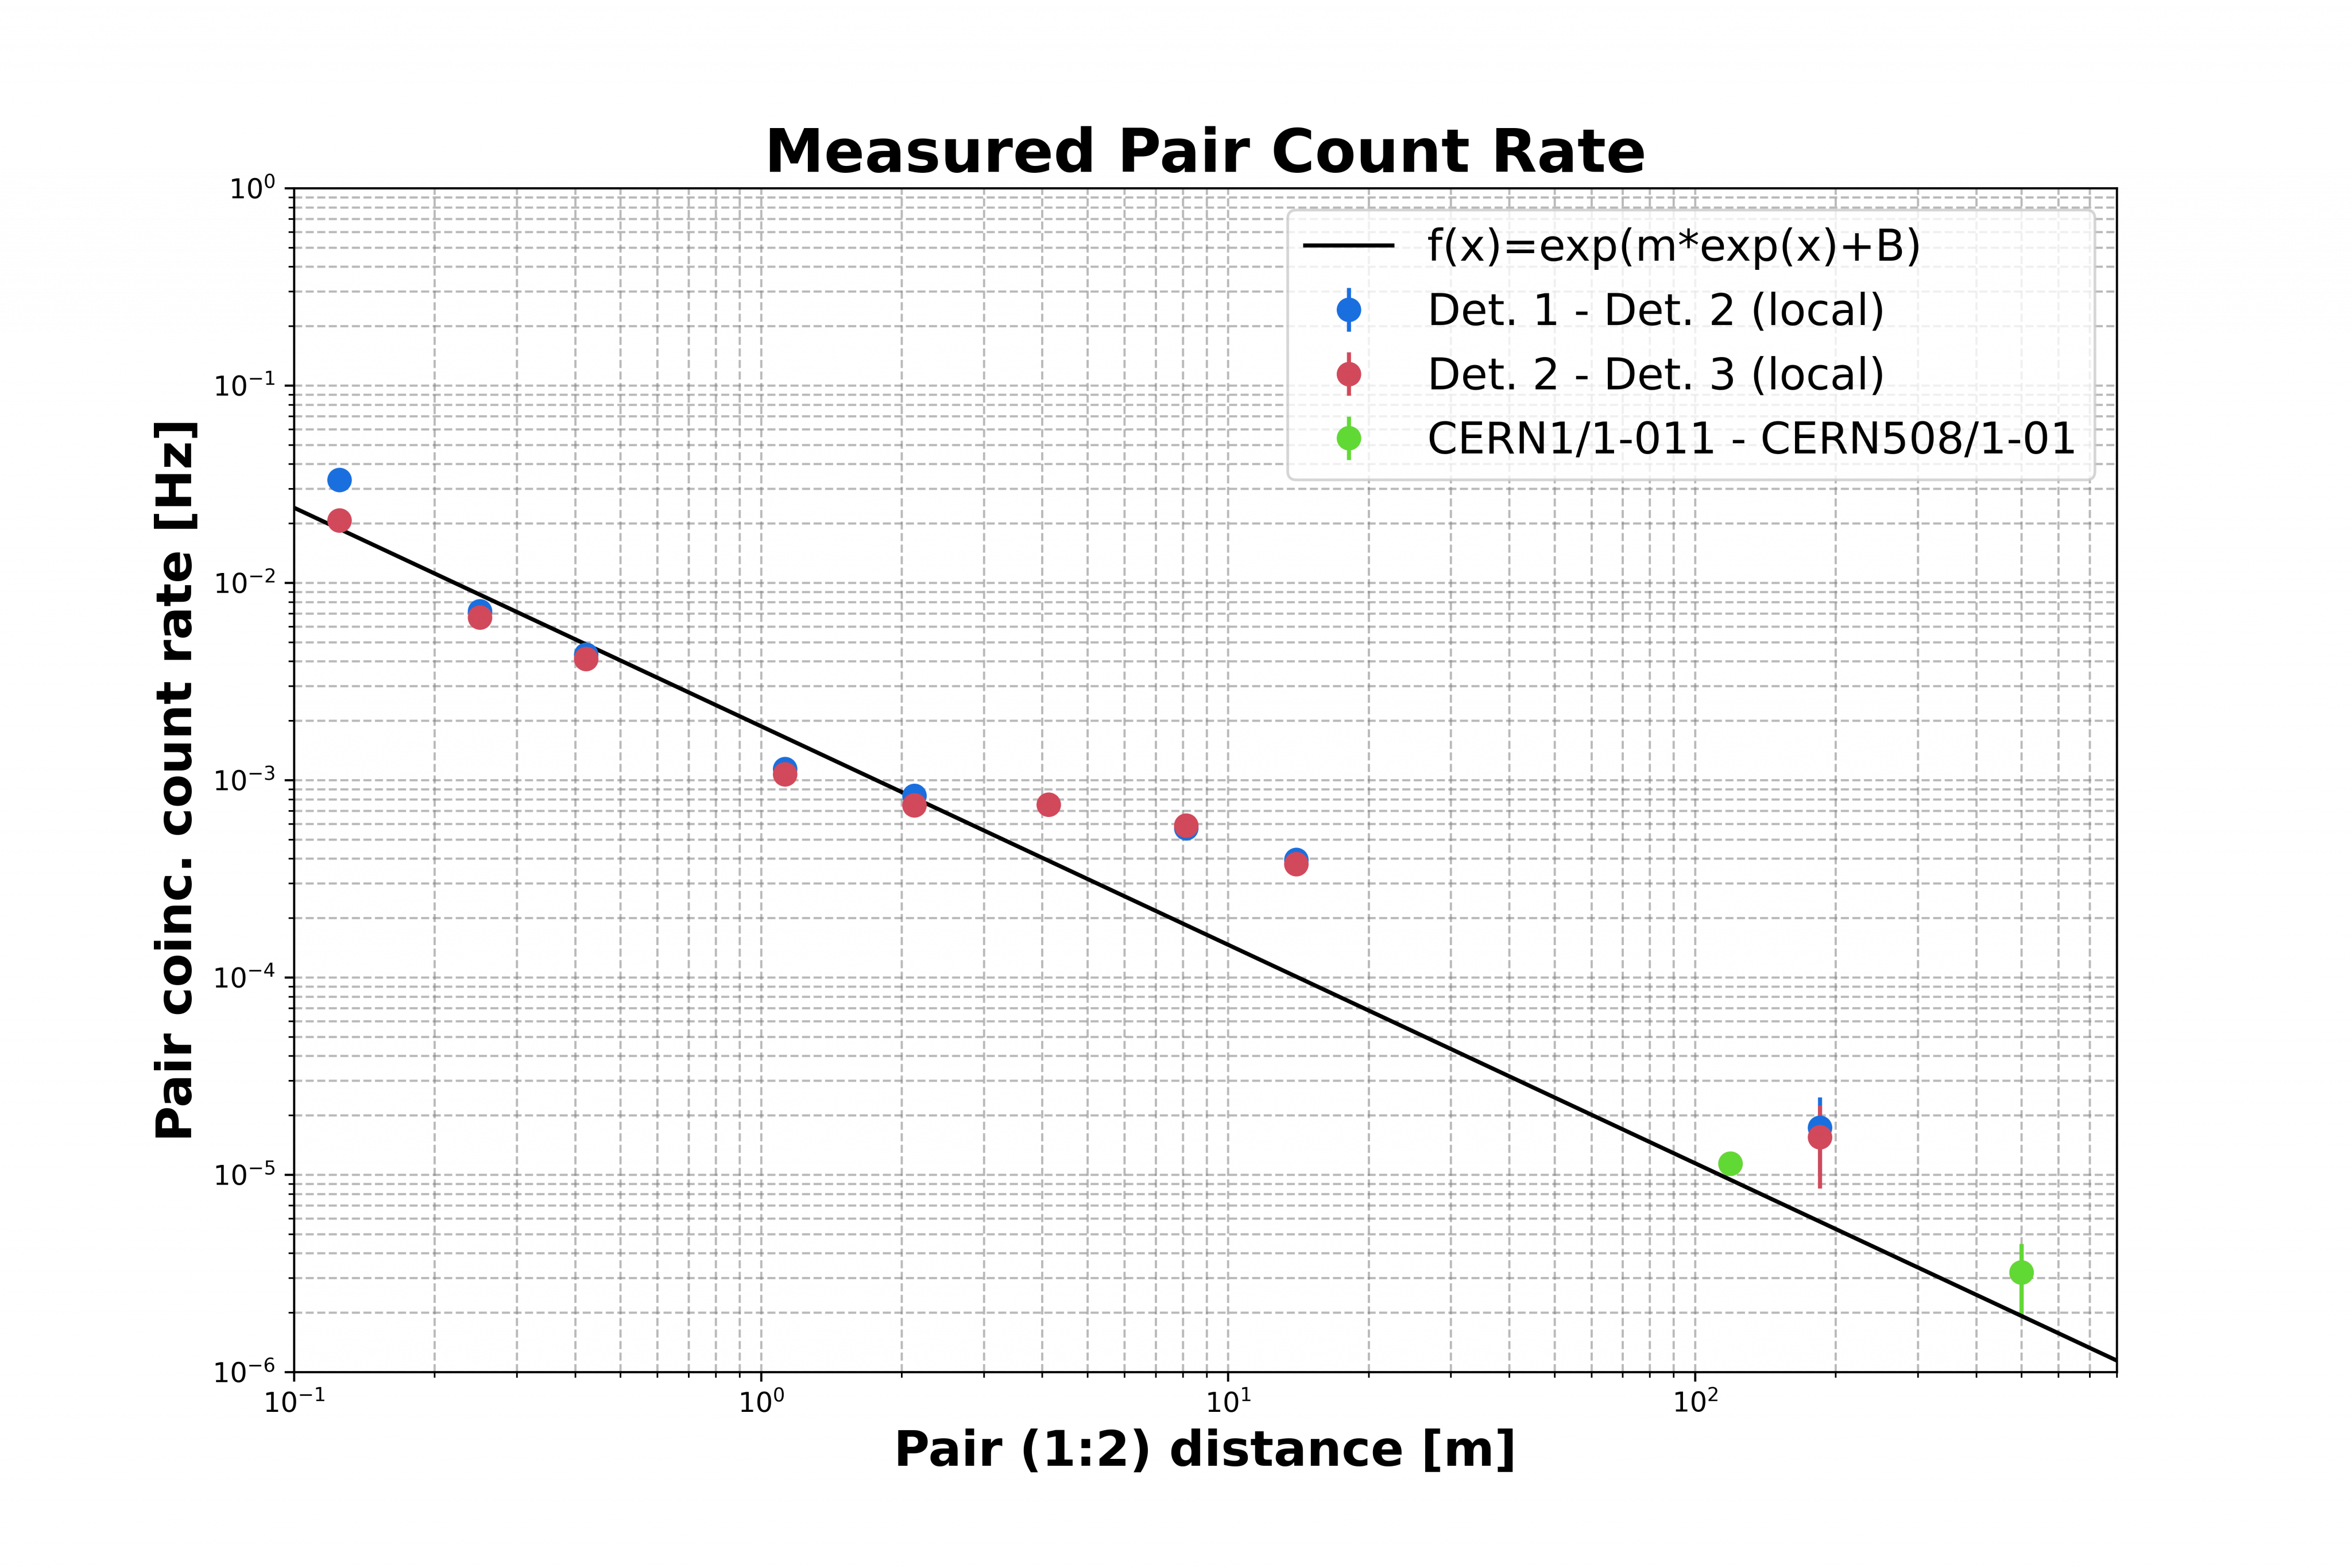
\includegraphics[width=0.7\linewidth]{data/pair-count-rate}
	\caption{Relationship between detector pair distance and coincidence rate\cite{muonpi}}
	\label{fig:pair-count-rate}
\end{figure}


\section{Real-time analysis}\label{sec:analysis}
In order to detect coincidences from all incoming single data points, each data point has to be compared with all others to find all possible combinations. To be able to do this, a useful criterium for a coincidence has to be found. A simple approach is to select a fixed maximum time difference which two events can have in order to be counted towards a coincidence. This however is inefficient and leads to large numbers of false positives, since a fixed interval can not perform well for detector combinations with large and short distances at the same time. Due to this a variable distance based criterium is used. For this purpose, the geodetic coordinates of both detector stations are taken and the straight line distance is calculated through \acrfull{enu} coordinates with the WGS84 model. The \acrshort{enu} coordinate system is a right handed local tangent plane carthesian coordinate system $\left(\hat{e}_{East},\hat{e}_{North},\hat{e}_{Up}\right)$ which is used to set different coordinates in relation to each other. The WGS84 model describes the shape of earth as an ellipsoid and provides reference measurements for this shape.
\begin{figure}[ht!]
	\centering
	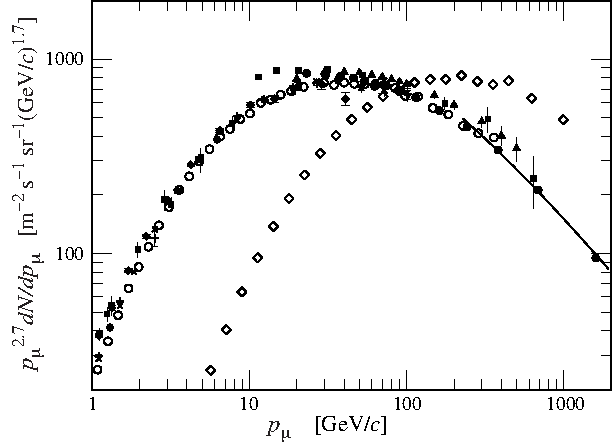
\includegraphics[width=0.7\linewidth]{data/cr_fig5_SeaLevelMuSpectra_09}
	\caption[Muon energy spectrum from vertical and inclined muons at sea level\cite{10.1093/ptep/ptaa104}]{Muon energy spectrum from vertical and inclined \tikz \draw[rotate=45] (0,0) rectangle(0.125,0.125); muons at sea level \cite[512]{10.1093/ptep/ptaa104}}
	\label{fig:muon-energy-spectrum}
\end{figure} \\
With this distance, the time of flight for the speed of light is calculated in order to receive the maximum physically viable time difference for one detector pair. This value however has large uncertainties especially for detector pairs which are close together.

Since there is a constant timing offset of a few nanoseconds for each detector pair which arises through the specific hardware setup, a minimum coincidence window must be defined to capture coincidences even for pairs with a large offset. A practical value of $150\,\text{ns}$ has been chosen.
It is also necessary to define an upper window, since the range of muons in air is limited and detector pairs with extremely large distances would create an abnormal and unphysical number of coincidences if left unconstrained. In order to find a useful upper limit for the coincidence window, the maximum possible flight distance for atmospheric muons has to be detemined. For that, the expected maximum range of muons in air is calculated. In order to do that, first a maximum expected energy is determined through the muon energy spectrum at sea level. Figure \ref{fig:muon-energy-spectrum} shows the muon energy spectrum at sea level for two different inclinations. A cutoff value of $10\,\text{TeV}$ is selected to calculate the maximum expected distance in air. Assuming the \acrfull{csda} range for a $10\,\text{TeV}$ muon taken from \cite{muon-range} of $7.634\cdot10^5\,\frac{\text{g}}{\text{cm}^2}$ and assuming standard condition air density of $1.225\,\frac{\text{kg}}{\text{m}^3}$, the maximum expected range of muons at sea level is $62.3\,\text{km}$. That equates to a time of flight of $207.87\,\mu\text{s}$ and thus a coincidence window of larger than that is not useful.
\subsection{Coincidence and plausability determination}\label{sec:coinc-calc}
In order to determine coincidences, each event needs to be checked against all other events which are currently in the event buffer. To determine whether two events contain a coincidence, it is beneficial to calculate a score for each pair as follows:
\begin{equation}\label{eq:coinc_score}
	c = 1 - \frac{|t_1 - t_2|}{t_{tof}}
\end{equation}
In equation \ref{eq:coinc_score} $t_1$ and $t_2$ denote the timestamps of both events and $t_{tof}$ the time of flight between both stations. This results in a number $c\leq1$ where a value $\leq0$ describes an unphysical coincidence.
\begin{figure}[ht!]
	\centering
	\begin{tikzpicture}
		\node (s1) [networknode] at (0, 0) {$s_1$};
		\node (s1r) [right=of s1] {};
		\node (s1b) [below=of s1] {};
		\node (s2) [networknode, below=of s1b] {$s_2$};
		\node (s3) [networknode, below right=of s1r] {$s_3$};
		\node (s3r) [below right=of s3] {};
		\node (s4) [networknode, below=of s3r] {$s_4$};
		
		\path[draw]
		(s1) edge node[left] {$c_{12}$} (s2)
		(s1) edge node[above] {$c_{13}$} (s3)
		(s2) edge node[left] {$c_{23}$} (s3)
		(s3) edge node[above right] {$c_{34}$} (s4)
		;
		\path[draw, dashed]
		(s1) edge node[below] {$c_{14}$} (s4)
		(s2) edge node[below] {$c_{13}$} (s4)
		;
		
		\draw[ultra thick, -> , >=latex] (4,0) -- ++(5,0) node[below] {$t$};
		\draw[dashed] (4.5,0.5) -- ++(0,-1) node[below] {$t_1$};
		\draw[dashed] (5.5,0.5) -- ++(0,-1) node[below] {$t_2$};
		\draw[dashed] (6.5,0.5) -- ++(0,-1) node[below] {$t_3$};
		\draw[dashed] (8,0.5) -- ++(0,-1) node[below] {$t_4$};
		
	\end{tikzpicture}
	\caption{Visualisation of four single events with possible coincidences}
	\label{fig:conflicts}
\end{figure} \\
In the case that multiple stations need to be compared, a complete graph needs to be calculated with edge weights equalling the score of the pair connected by this edge. An example of this construction is shown in figure \ref{fig:conflicts}.
There, \tikz \draw (0,0) -- (0.5,0); marks a physical time difference and \tikz \draw[dashed] (0,0) -- (0.5,0); marks an unphysical time difference. This leads to a conflict, since all stations $s_{1,2,3,4}$ have at least one physical coincidence time to at least one other station, but the data for $s_4$ only fits together with the data of $s_3$. This means that the whole coincidence is not physically viable, though an unknown number of partial coincidences can be.

In order to quantify this problem as one number, the unweighted plausibility score is introduced. Consider the graph with vertices $V = (s_1; s_2; s_3; s_4)$ from figure \ref{fig:conflicts} where the edges describe possible coincidences and the vertices detector stations. Only the set of edges $E = (c_{12}; c_{13}; c_{23}; c_{24})$ contains valid coincidences. The plausibility score of a full event with $n$ detector stations is then defined through
\begin{equation}
p = \frac{|E|}{\Delta_{n-1}}=\frac{2\cdot|E|}{n(n-1)}
\end{equation}
where $\Delta_n$ is the triangular number and $|E|$ the number of edges in the set $E$.

For a fully plausible coincidence event, this score is $1$, for the example in figure \ref{fig:conflicts} it is $p = \frac{4}{6}=\frac{2}{3}$.

In order to attempt to resolve this conflict additionally the weighted plausibility score $_wp$ is introduced:
\begin{equation}
	_wp = \frac{\sum^{n}_{i}\sum^{n}_{j} c_{ij}}{\Delta_{n-1}}
\end{equation}

The goal in resolving conflicting data is to maximise $_wp$ and reach $p=1$. Without access to more data is is impossible to definitively resolve this conflict, however an approximation can be performed.

This approximation can be done through selectively removing the vertex $s_i$ with lowest weighted rank
\begin{equation}
_wrank(s_i) = \sum_{j}^{n}c_{ij}
\end{equation}
in the graph and recalculating $_wp$, this is repeated until $p=1$ is reached. Should this prove to be impossible without removing too many edges for the purpose of preserving potentially useful data the process is cancelled and the whole event is accepted tentatively.

\subsection{Reconstruction of possible primary incident angles} \label{sec:reconstruction}
Through the assumptions shown in figure \ref{fig:angle-assumptions}, the possible source directions of a primary particle can be reduced. There, the geometry of a coincidence with $n=2$ is shown.
\begin{figure}[ht!]
	\centering
	\begin{tikzpicture}
		\fill (0,0) coordinate(det1) circle(0.1);
		\fill (6,0) coordinate(det2) circle(0.1);
		\draw (det2) circle(1);
		\draw (det2) -- ++(125:0.7) node[right] {$\ell$} -- ++(125:6.4) coordinate(center);
		\draw[dashed] (det2) ++(125:1) ++ (215:2) -- ++(35:4) node[right] {tangent};
		\draw (det2) ++ (125:1) arc(-55:-35:6.1) arc(-35:-125:6.1) node[left] {shower front};
		\draw (center) -- (det1) -- (det2);
		\draw (det2) ++(125:1) -- (det1);
		\draw (det2) ++(125:1) -- ++(0,1) -- ++(0,-2);
		
		\draw (det1) -- ++(0,-0.9) coordinate(det1b) -- ++(0,-0.1);
		\draw (det2) -- ++(0,-0.9) coordinate(det2b) -- ++(0,-0.1);
		
		\draw[<->] (det2b) -- (det1b);
		\node[above] at ($(det1b)!0.5!(det2b)$) {$d$};
		\node[above left] at ($(det1)!0.5!(center)$) {$r$};
		
		\draw[<->] (center) ++(-55:2) arc(-55:-108:2) node[midway, above] {$\delta$};
		\draw[<->] (det2) ++(125:2) arc(125:90:1) node[midway, above] {$\alpha$};
		\draw[<->] (det2) ++(125:2) arc(125:189:1) node[midway, left] {$\gamma$};
		\draw[<->] (det1) ++(0:1) arc(0:72:1) node[midway, above right] {$\phi$};
		\draw[<->] (det1) ++(0:3) arc(0:8.584336297778657:3) node[midway, right] {$\beta$};
		\draw[<->] (det1) ++(8.584336297778657:3) node[above] {$s$};
		
	\end{tikzpicture}
	\caption{Assumption for possible incidence angles}
	\label{fig:angle-assumptions}
\end{figure} \\
Since the shower front can be simplified as a spherical cap and the propagation speed can be assumed to be near the speed of light, two spheres with a shared tangent can be constructed. One spherical surface is the shower front, the other is a sphere around the detector which had the later event timing. Its radius $\ell$ is equal to the propagation time of light for the coincidence time. Through geometrical analysis of this arrangement, the radius and angle pair can be derived as a function of the angle $\alpha$. This creates a curve in the plane on which the primary interaction must have taken place. Due to the symmetry of this arrangement however, in 3-D space, this curve becomes a rotational surface. \\
In the case of a coincidence with $n>2$ multiple curves can be calculated relative to the same root detector. This allows for the intersection points of each rotational surface to be calculated, which results in a reduced possible origin area for the primary interaction. \\
Given that the shower front is not a complete spherical surface but only a spherical cap, the possible origin directions can be reduced with this approach. In the case of higher coincidence numbers, the possible direction can be reduced further. Additionally to the possible directions, this approach also provides a lower limit for the shower radius and footprint radius, suggesting a minimum Particle energy.
Calculating the angles $\beta$ and $\gamma$ and length $s$, the equations
\begin{equation*}
	\beta = \arctan\left(\frac{\ell\cdot\cos\alpha}{d - \ell\sin\alpha}\right),
\end{equation*}
\begin{equation*}
	\gamma = \frac{\pi}{2} - \alpha + \beta
\end{equation*}
and
\begin{equation*}
	s = \sqrt{\left(l\cdot\cos\hspace{-2pt}\left(\alpha\right)\right)^2 + \left(d - l\cdot\sin\left(\alpha\right)\right)^2} = \sqrt{l^2 + d^2 - 2dl\sin\left(\alpha\right)}
\end{equation*}
can be derived. With those, the polar coordinates $(\phi, r)$ can be calculated with equations \ref{eq:phi} and \ref{eq:r}.
\begin{equation}\label{eq:phi}
	\phi = \gamma + \beta = \frac{\pi}{2} - \alpha + 2\cdot\beta
\end{equation}
\begin{equation}\label{eq:r}
	r = \frac{s}{2\cdot\cos\left(\gamma\right)} = \frac{\sqrt{l^2 + d^2 - 2{\cdot}d{\cdot}l{\cdot}\sin\left(\alpha\right)}}{2\cdot\sin\left(\alpha - \beta\right)}
\end{equation}


Figure \ref{fig:reconstruction_example} shows an example for possible combinations of $r$ and $\phi$ as calculated above for a detector pair with distance of $3.4\,\text{km}$ and a coincidence time of $7.37\,\mu\text{s}$. Following the curve, the free parameter $\alpha$ is varied. The minimum possible distance is reached when $\alpha=\frac{\pi}{2}$, since then the center of the constructed circle in figure \ref{fig:angle-assumptions} lies directly on the line between both detectors. As $\alpha$ approaches $0$, the possible radius tends to infinity and $\phi$ tends to a stationary value $\phi_\infty$.
\begin{figure}[ht!]
	\centering
	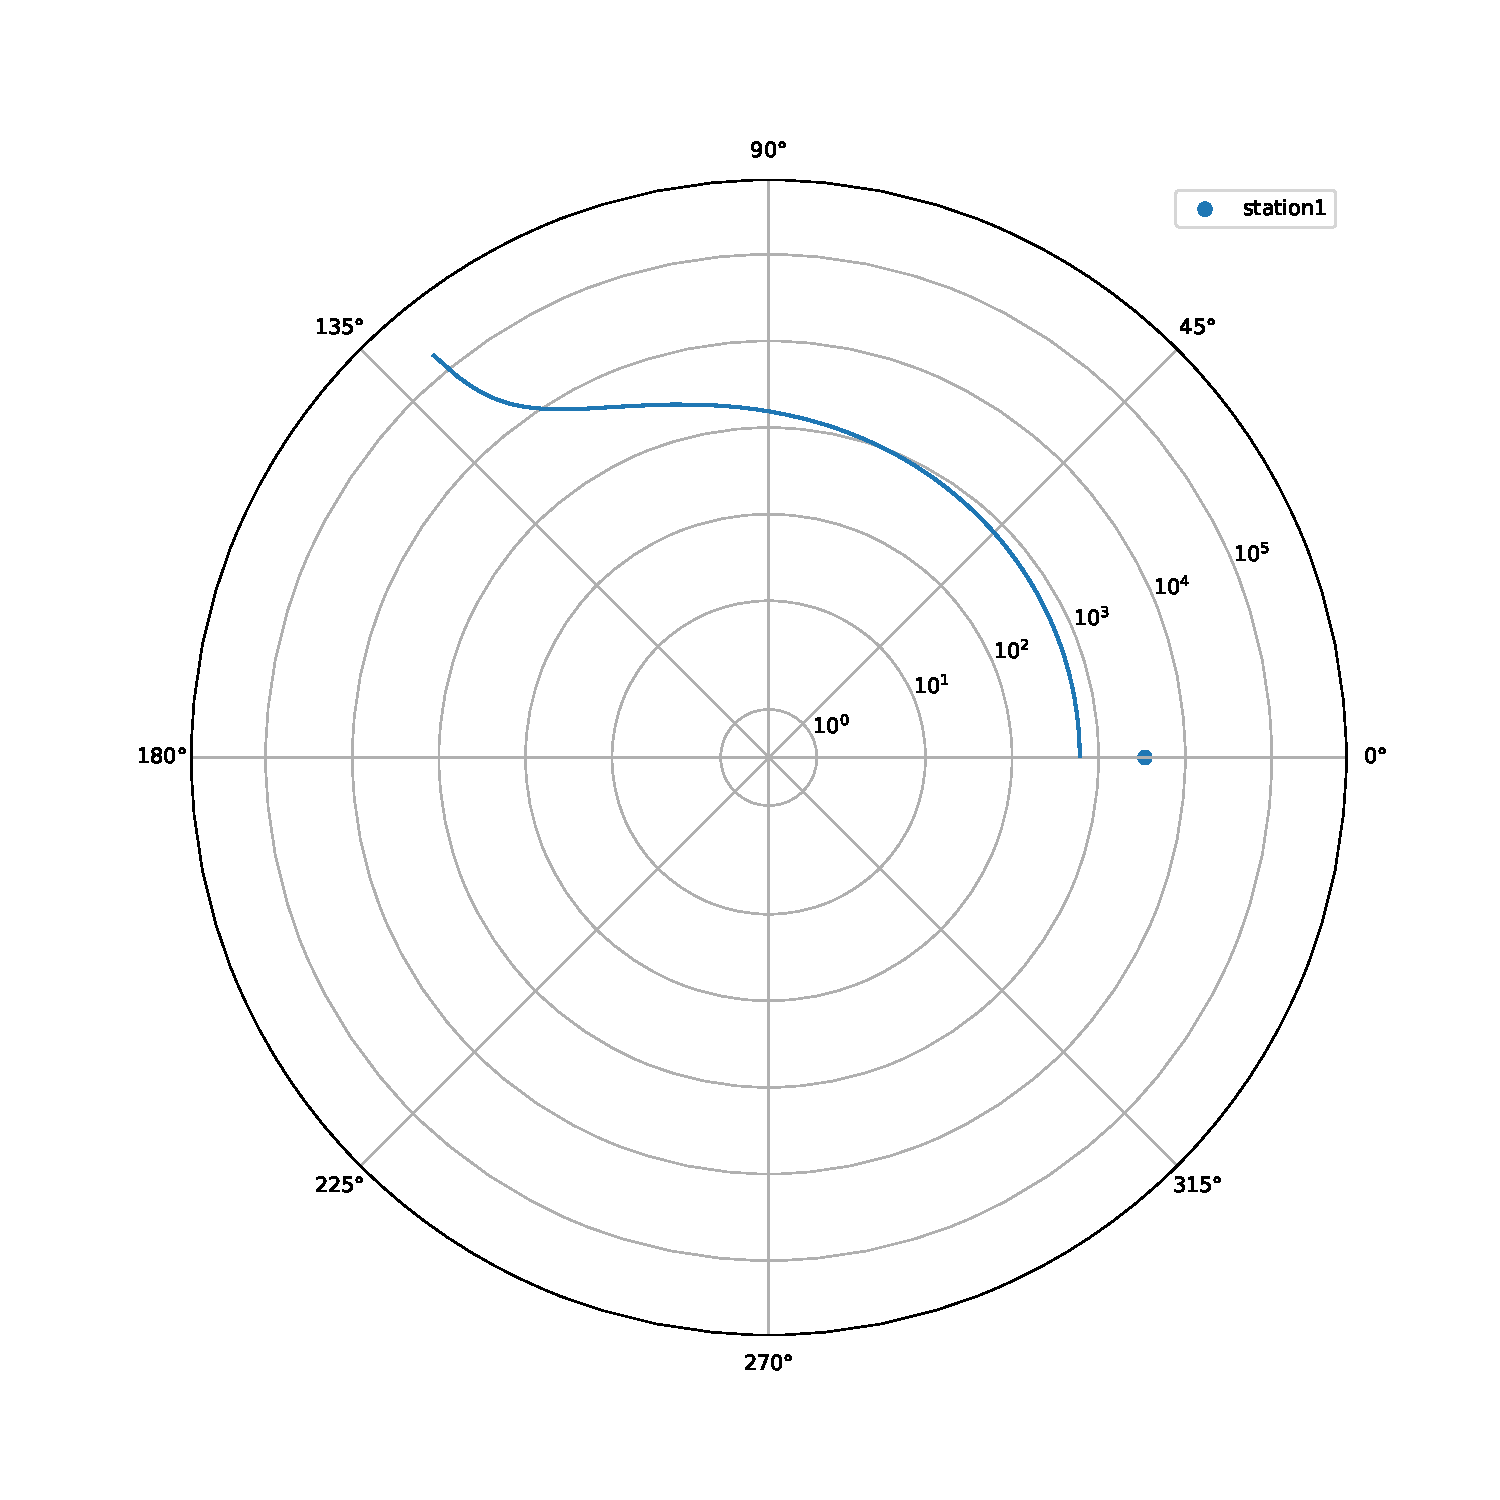
\includegraphics[width=0.4\linewidth]{data/example_plot_vertical}
	\caption{Plot of an example to reconstruct the possible direction of incident primary particle}
	\label{fig:reconstruction_example}
\end{figure}
\begin{equation*}
	\begin{aligned}
		\lim_{\alpha\rightarrow0}r\left(\alpha\right) &= \infty\\
		\lim_{\alpha\rightarrow0}\phi\left(\alpha\right) &= \phi_\infty
	\end{aligned}
\end{equation*}
Noteworthy is that the possible values for $\alpha$ are constrained by a maximum value for $\delta$ due to a maximum shower footprint on earth. Adjusting for that, a lower limit for the radius r can be calculated iteratively through equation \ref{eq:delta_alpha}.
\begin{equation}\label{eq:delta_alpha}
	\delta = \pi - 2\cdot\gamma = 2\cdot\alpha - 2\cdot\arctan\left(\frac{\ell\cdot\cos\alpha}{d - \ell\sin\alpha}\right)
\end{equation}
\begin{figure}[ht!]
	\centering
	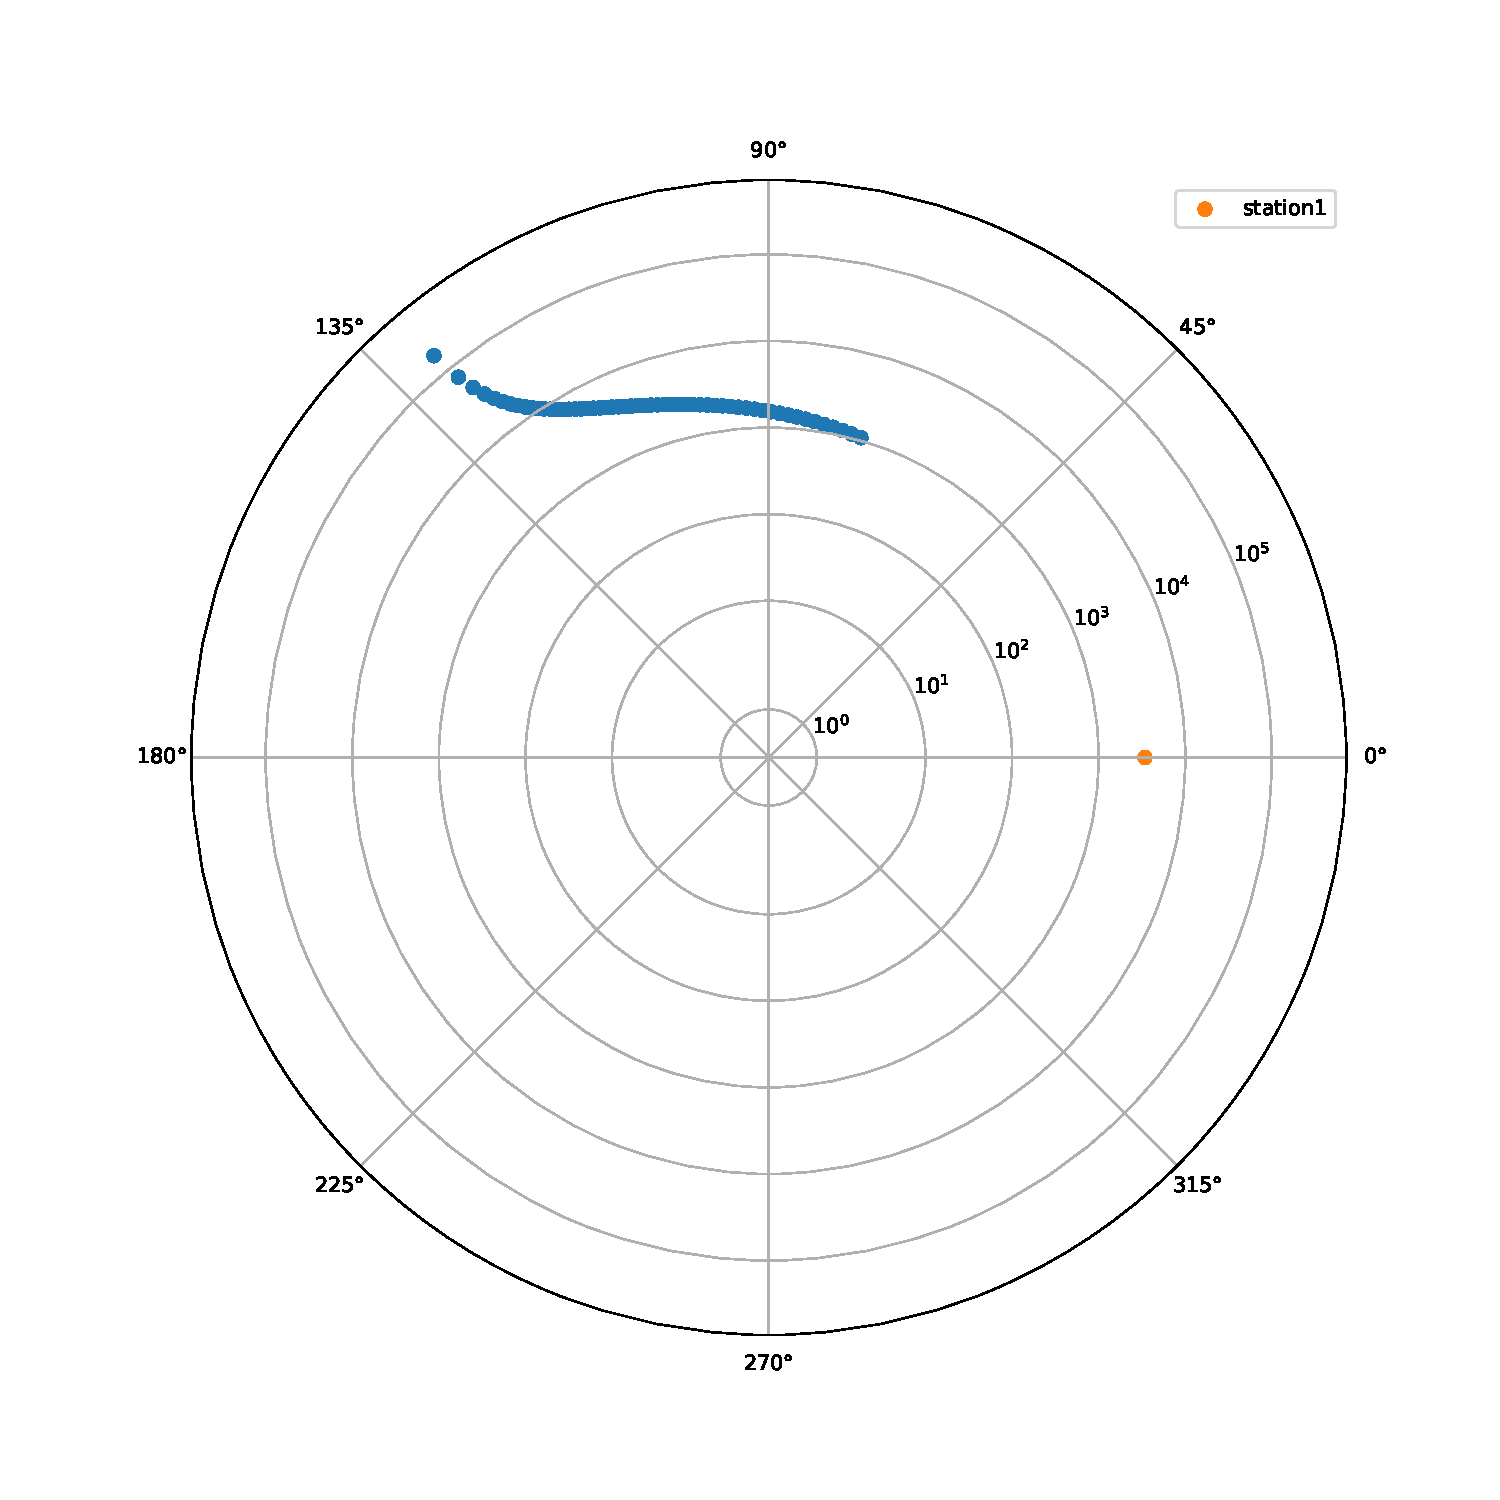
\includegraphics[width=0.4\linewidth]{data/example_plot_vertical_constrained}
	\caption{Possible incident angles and radii constrained to a maximum possible angle $\delta_{max}$}
	\label{fig:reconstruction_example_constrained}
\end{figure}
Figure \ref{fig:reconstruction_example_constrained} shows the same plot as figure \ref{fig:reconstruction_example} but with a constrained angle $\delta_{max} = \frac{\pi}{4}$.

Due to the inherent rotational symmetry of the system around the connecting straight line between both detectors, the curve shown in figures \ref{fig:reconstruction_example} and \ref{fig:reconstruction_example_constrained} show the outline of a rotational body with rotational axis equal to the connecting line. This permits a projection of the curve onto the ground in either direction. Doing this, the curves for all pairs involving a reference detector station can be calculated and projected onto the same plot, aligned according to the real world positions.
\begin{figure}[ht!]
	\centering
	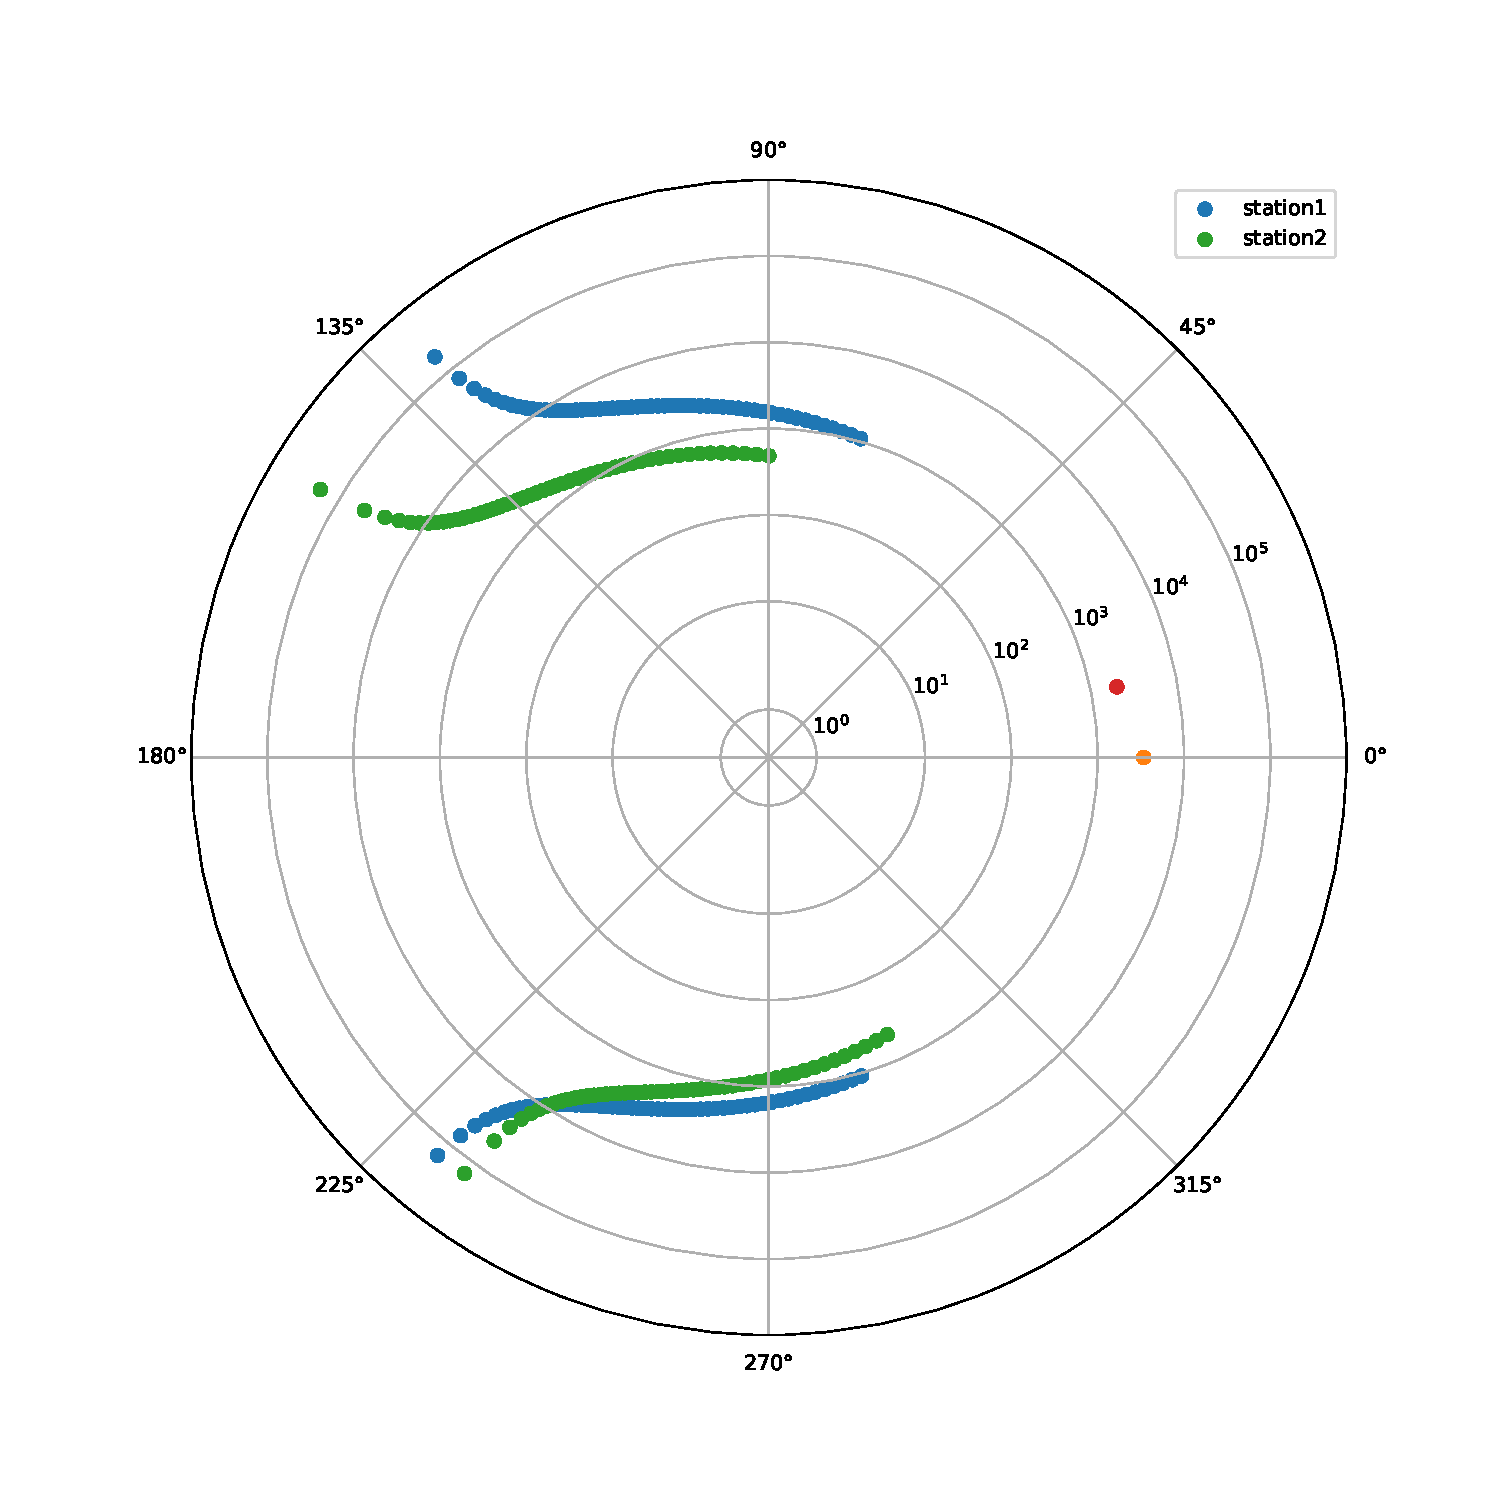
\includegraphics[width=0.4\linewidth]{data/example_plot_ground}
	\caption{Ground plot for a coincidence with $n=3$.}
	\label{fig:reconstruction_example_ground}
\end{figure}\\
Figure \ref{fig:reconstruction_example_ground} shows this construction for a coincidence $n=3$, where the reference detector is located in the center and both other detectors are located towards the right. The real world distance between the reference station and station1 is $3.4\,\text{km}$, between the reference and station2 $2\,\text{km}$.
It can be seen that the curves overlap in the bottom half of the plot, indicating a possible origin region for the primary interaction.


Though due to the fact that the space of possible origin points is a rotational body, the cross section between both curves is a region in 3D space.
\section{Program layout}
The analysis program uses a data driven pipeline design for efficient execution. This is an approach where the processing units in the software do not continuously poll for data but only get called once data is available. Though for time critical applications, a maximum waiting time is defined after which the processing unit is invoked.

Apart from processing all events, it takes over the task of supervision of itself and all detector stations. For the purpose of keeping track of internal changes and changes in detector station status, a trigger system is employed in order to receive status updates outside of the application.
Periodically it stores runtime information and detector states in a database.
An overview of the program layout for the real-time analysis is shown in Figure \ref{fig:programlayout}, the parts marked with section numbers are described in detail in their respective sections.
\begin{figure}[h!]
	\centering
	\begin{tikzpicture}[->]
		\node (source) [draw, terminal,minimum height=1cm] {Event source};
		\node (logsource) [left=of source, draw, terminal,minimum height=1cm] {Station log source};
		\node (supervision) [below=of source, draw, process,minimum height=1cm] {Station supervision (\ref{subsec:station-s})};
		\node (supervision2) [below=of supervision, draw, process,minimum height=1cm] {Time-base supervision (\ref{subsec:timebase-s})};
		\node (filter) [below=of supervision2, draw, process,minimum height=1cm] {Coincidence filter (\ref{subsec:coincidence-f})};
		\node (analysis) [right=of filter, draw, process,minimum height=1cm] {Coincidence analysis (\ref{subsec:coincidence-s})};
		\node (sink) [below=of filter, draw, terminal,minimum height=1cm] {Event Sink};

		\node (criterium) [left=of filter, draw, predproc,minimum height=1cm] {Coincidence criterium};
		
		\draw (logsource) |- (supervision);
		\draw (source) -- (supervision);
		\draw (supervision) -- (supervision2);
		\draw (supervision2) -- (filter);
		\draw (filter) -- (sink);
		\draw (filter) -- (analysis);
		\draw (supervision) -| (analysis);
		
		\draw[<->] (criterium) -- (filter);
	\end{tikzpicture}
	\caption{Program layout}
	\label{fig:programlayout}
\end{figure} \\

The station log source and event source are abstract classes which can be implemented through multiple different protocols, though at the moment only a \acrshort{mqtt} implementation is used. The same is true for the Even Sink class, though there are three distinct implementations available. The first is a sink for use with an influxDB database which is used per default. Additionally there is a debugging sink which uses text output onto the console and the third is a sink to \acrshort{mqtt} which can be used if the application should be used as an instance for a local arrangement for a few detectors. This local instance then sends the processed data along to the next instance, effectively performing a preprocessing step for dense local arrangements.
\subsection{Station supervision}\label{subsec:station-s}
The station supervision tracks all currently active detector stations and classifies them according to reliable and unreliable data states.
Additionally it augments each event with the location and user data which is not provided with the default event messages.
\begin{figure}[h!]
	\centering
	\begin{tikzpicture}[->]
		\node (start) at (0,0) {};
		\node (terminal1) [below=of start,draw, terminal] {event input};
		\node (predproc1) [below=of terminal1, draw, predproc, align=left] {calculate event rate};
		\node (decide1) [below=of predproc1, draw, decision] {$\sigma\geq{k}\cdot\mu$};
		\node (terminal2) [right=of start, draw, terminal] {station log input};
		\node (decide2) [below right=of terminal2, draw, decision] {$\bar{f}_{loc}\geq1$};
		\node (decide3) [right=of predproc1, draw, decision] {$\bar{f}_{time}\geq1$};
		\node (predproc2) [below=of decide1, draw, terminal, align=left] {Mark station unreliable};
		
		
		\draw (terminal1) -- (predproc1);
		\draw (predproc1) -- (decide1);
		\draw (decide1) -- (predproc2);
		\draw (terminal2) -| (decide2);
		\draw (terminal1) -| (decide3);
		\draw (decide2) |- (predproc2);
		\draw (decide3) |- (predproc2);
	\end{tikzpicture}
	\caption{Criteria for detector station reliability}
	\label{fig:station_reliability}
\end{figure}
Figure \ref{fig:station_reliability} shows the decision process how each station is determined to be reliable. Each event is analysed and the mean event rate as well as the standard deviation of the rate is calculated continuously. If $\sigma\geq{k}\cdot\mu$ is true, where $\sigma$ is the standard deviation of the rate, $\mu$ the mean rate and $k$ a constant, the detector station is determined to have a highly unstable rate and is excluded from contributing events to the analysis.

Additionally two more factors can determine the reliability of a station. Those factors are normed so that a value of higher than 1 causes an unreliability mark.
$\bar{f}_{time}$ is the mean time accuracy and $\bar{f}_{loc}$ the mean location precision of the \acrshort{gnss} receiver.

The time accuracy is determined through the detector station itself and results from different factors such as the \acrshort{gnss} signal quality.
The location precision is calculated through
\begin{equation*}
loc = dop\cdot\sqrt{h_{acc}^2 + v_{acc}^2}
\end{equation*}
where $dop$ is the delusion of precision, $h_{acc}$ the horizontal and $v_{acc}$ the vertical accuracy of the \acrshort{gnss} receiver. All those values are also determined in each detector station for itself.

For all determining factors, a hysteresis is used in order to provide a more stable status of each detector station.
\begin{figure}[ht!]
	\centering
	\begin{tikzpicture}[->]
		\node (terminal1) at (0,0) [draw, terminal] {event input};
		\node (decide1) [below=of terminal1, draw, decision] {detector known};
		\node (decide2) [below=of decide1, draw, decision] {detector reliable};
		\node (decide3) [below=of decide2, draw, decision] {$f_{time}\gg1$};
		\node (predproc1) [below=of decide3, draw, predproc, align=left] {Add location info};
		\node (terminal2) [below=of predproc1, draw, terminal] {pass to coincidence filter};
		
		\node (decide1r) [right=of decide1] {no};
		\node (decide2r) [right=of decide2] {no};
		\node (decide3r) [right=of decide3] {yes};
		
		\node (terminal3) [right=of decide2r, draw, terminal] {discard event};
		
		
		
		\draw (terminal1) -- (decide1);
		\draw (decide1) -- (decide2);
		\draw (decide2) -- (decide3);
		\draw (decide3) -- (predproc1);
		\draw (predproc1) -- (terminal2);
		\draw (decide1) -- (decide1r) -| (terminal3);
		\draw (decide2) -- (decide2r) -- (terminal3);
		\draw (decide3) -- (decide3r) -| (terminal3);
	\end{tikzpicture}
	\caption{Path of an event through the station supervisor}
	\label{fig:event_station_supervisor}
\end{figure}
In figure \ref{fig:event_station_supervisor} the path of an event through the station supervisor is shown. There, only events which can be attributed to a reliable detector are accepted. Additionally, events where the time accuracy reaches extreme values are automatically discarded, since the method shown before in figure \ref{fig:station_reliability} has some inertia. This can cause single events with extremely inaccurate timestamps to artificially increase the time-base to extreme values.
\subsection{Time-base supervision}\label{subsec:timebase-s}
Since the detector network is so widely distributed, network lag and outages can introduce considerate deviations in arrival times between event messages from different detector stations. Consider the scenario shown in figure \ref{fig:network-topology}. There detector stations $A$, $B$ and $C$ all have different network delays to the server and so the event timestamps marked with $t_{A,B,C}$ have different arrival times at the server marked as $t'_{A,B,C}$. That necessitates a considerably larger sample interval for the coincidence determination than the expected coincidence interval.
\begin{figure}[ht!]
	\centering
	\begin{tikzpicture}
		\node (server) [networknode] at (6.5,5) {Server};
		\node (serverbl) [below left=of server] {};
		\node (serverbr) [below right=of server] {};
		\node (servera) [above=of server] {};
		\node (a) [networknode, above=of servera] {A};
		\node (b) [networknode, below right=of serverbr] {B};
		\node (c) [networknode, below left=of serverbl] {C};
		
		\path[draw]
			(a) edge node[left] {$100\,\text{ms}$} (server)
			(b) edge node[above right] {$10\,\text{ms}$} (server)
			(c) edge node[left] {$35\,\text{ms}$} (server)
			;
			
			\draw[decoration={%
				discontinuity,
				amplitude=5,
				meta-segment length=2,
				segment length=3},
			decorate, ultra thick] (0,0) -- (10,0);
			\draw[ultra thick, ->] (10,0) -- (13,0) node[below] {$t$};
			\draw[dashed] (1,0.5) -- ++(0,-1) node[below] {$t_A$};
			\draw[dashed] (3,0.5) -- ++(0,-1) node[below] {$t_B$};
			\draw[dashed] (4,0.5) -- ++(0,-1) node[below] {$t_C$};
			
			\draw[dashed] (6,0.5) -- ++(0,-1) node[below] {$t_B'$};
			\draw[dashed] (7,0.5) -- ++(0,-1) node[below] {$t_C'$};
			\draw[dashed] (10,0.5) -- ++(0,-1) node[below] {$t_A'$};
	\end{tikzpicture}
	\caption{Network topology of detector network}
	\label{fig:network-topology}
\end{figure}

The time-base supervisor determines a baseline waiting interval by observing the maximum time difference between event timestamps over a certain sample time interval. A value of $2\,\text{s}$ proved experimentally to provide a good balance between runtime impact, stability and reaction time. In the case of a total network outage for one detector station however, the events will be buffered locally in the station and transmitted at a later time when the network connection has been re-established. This can mean delays of up to a few minutes and would lie outside the two second time-base and a loss of data would be the result. In order to mitigate this, an attempt to predict network outages is implemented by observing the current event rate in relation to the mean event rate over a long sample time. A factor is calculated through
\begin{equation*}
	f = max(1, \frac{\mu_{r} - r}{\sigma_{r}})
\end{equation*}
where $r$ is the current event rate, $\mu_{r}$ the mean rate and $\sigma_{r}$ the standard deviation of the rate over a long sample time. This factor is then relative to the expected event rate of the detector station and is always greater or equal to 1. This is calculated for all detector stations and the maximum value is used as a scaling factor for the previously described time-base.
\clearpage
The resulting time value can then be used by the coincidence filter as a timeout value for the construction of coincidence events.

\begin{figure}[ht!]
	\centering
	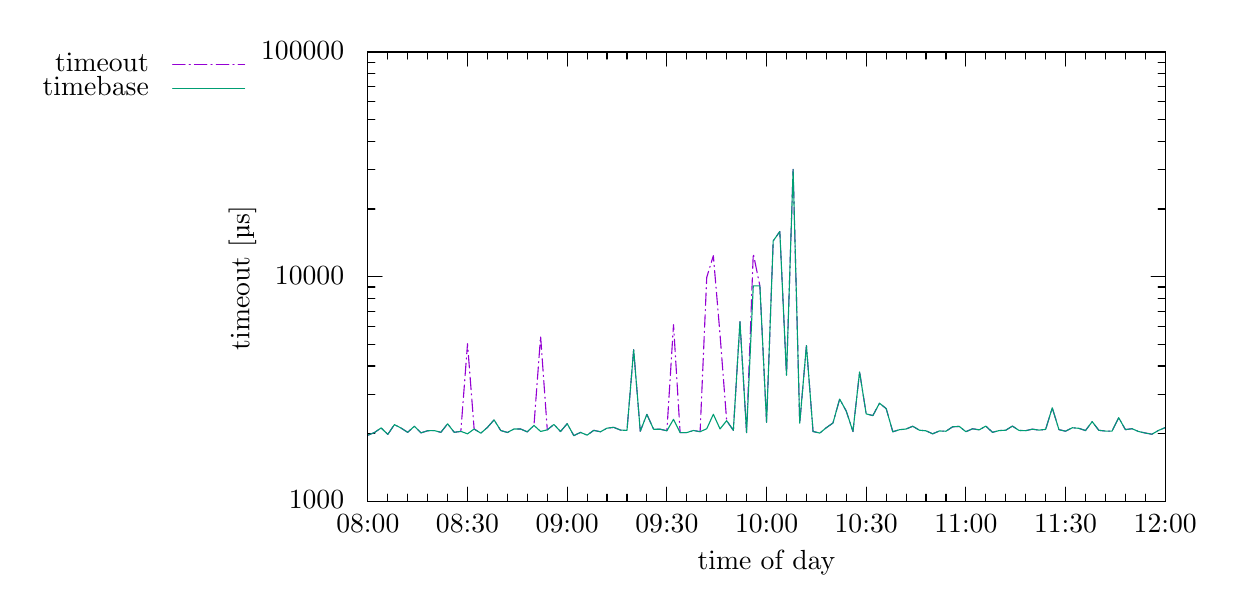
\begin{tikzpicture}[gnuplot]
%% generated with GNUPLOT 5.4p1 (Lua 5.4; terminal rev. Jun 2020, script rev. 114)
%% Mon 19 Jul 2021 16:30:23
\path (0.000,0.000) rectangle (15.000,7.000);
\gpcolor{color=gp lt color border}
\gpsetlinetype{gp lt border}
\gpsetdashtype{gp dt solid}
\gpsetlinewidth{1.00}
\draw[gp path] (4.320,0.985)--(4.500,0.985);
\draw[gp path] (14.447,0.985)--(14.267,0.985);
\node[gp node right] at (4.136,0.985) {$1000$};
\draw[gp path] (4.320,1.844)--(4.410,1.844);
\draw[gp path] (14.447,1.844)--(14.357,1.844);
\draw[gp path] (4.320,2.346)--(4.410,2.346);
\draw[gp path] (14.447,2.346)--(14.357,2.346);
\draw[gp path] (4.320,2.703)--(4.410,2.703);
\draw[gp path] (14.447,2.703)--(14.357,2.703);
\draw[gp path] (4.320,2.979)--(4.410,2.979);
\draw[gp path] (14.447,2.979)--(14.357,2.979);
\draw[gp path] (4.320,3.205)--(4.410,3.205);
\draw[gp path] (14.447,3.205)--(14.357,3.205);
\draw[gp path] (4.320,3.396)--(4.410,3.396);
\draw[gp path] (14.447,3.396)--(14.357,3.396);
\draw[gp path] (4.320,3.562)--(4.410,3.562);
\draw[gp path] (14.447,3.562)--(14.357,3.562);
\draw[gp path] (4.320,3.707)--(4.410,3.707);
\draw[gp path] (14.447,3.707)--(14.357,3.707);
\draw[gp path] (4.320,3.838)--(4.500,3.838);
\draw[gp path] (14.447,3.838)--(14.267,3.838);
\node[gp node right] at (4.136,3.838) {$10000$};
\draw[gp path] (4.320,4.697)--(4.410,4.697);
\draw[gp path] (14.447,4.697)--(14.357,4.697);
\draw[gp path] (4.320,5.199)--(4.410,5.199);
\draw[gp path] (14.447,5.199)--(14.357,5.199);
\draw[gp path] (4.320,5.556)--(4.410,5.556);
\draw[gp path] (14.447,5.556)--(14.357,5.556);
\draw[gp path] (4.320,5.832)--(4.410,5.832);
\draw[gp path] (14.447,5.832)--(14.357,5.832);
\draw[gp path] (4.320,6.058)--(4.410,6.058);
\draw[gp path] (14.447,6.058)--(14.357,6.058);
\draw[gp path] (4.320,6.249)--(4.410,6.249);
\draw[gp path] (14.447,6.249)--(14.357,6.249);
\draw[gp path] (4.320,6.415)--(4.410,6.415);
\draw[gp path] (14.447,6.415)--(14.357,6.415);
\draw[gp path] (4.320,6.560)--(4.410,6.560);
\draw[gp path] (14.447,6.560)--(14.357,6.560);
\draw[gp path] (4.320,6.691)--(4.500,6.691);
\draw[gp path] (14.447,6.691)--(14.267,6.691);
\node[gp node right] at (4.136,6.691) {$100000$};
\draw[gp path] (4.320,0.985)--(4.320,1.165);
\draw[gp path] (4.320,6.691)--(4.320,6.511);
\node[gp node center] at (4.320,0.677) {08:00};
\draw[gp path] (4.573,0.985)--(4.573,1.075);
\draw[gp path] (4.573,6.691)--(4.573,6.601);
\draw[gp path] (4.826,0.985)--(4.826,1.075);
\draw[gp path] (4.826,6.691)--(4.826,6.601);
\draw[gp path] (5.080,0.985)--(5.080,1.075);
\draw[gp path] (5.080,6.691)--(5.080,6.601);
\draw[gp path] (5.333,0.985)--(5.333,1.075);
\draw[gp path] (5.333,6.691)--(5.333,6.601);
\draw[gp path] (5.586,0.985)--(5.586,1.165);
\draw[gp path] (5.586,6.691)--(5.586,6.511);
\node[gp node center] at (5.586,0.677) {08:30};
\draw[gp path] (5.839,0.985)--(5.839,1.075);
\draw[gp path] (5.839,6.691)--(5.839,6.601);
\draw[gp path] (6.092,0.985)--(6.092,1.075);
\draw[gp path] (6.092,6.691)--(6.092,6.601);
\draw[gp path] (6.345,0.985)--(6.345,1.075);
\draw[gp path] (6.345,6.691)--(6.345,6.601);
\draw[gp path] (6.599,0.985)--(6.599,1.075);
\draw[gp path] (6.599,6.691)--(6.599,6.601);
\draw[gp path] (6.852,0.985)--(6.852,1.165);
\draw[gp path] (6.852,6.691)--(6.852,6.511);
\node[gp node center] at (6.852,0.677) {09:00};
\draw[gp path] (7.105,0.985)--(7.105,1.075);
\draw[gp path] (7.105,6.691)--(7.105,6.601);
\draw[gp path] (7.358,0.985)--(7.358,1.075);
\draw[gp path] (7.358,6.691)--(7.358,6.601);
\draw[gp path] (7.611,0.985)--(7.611,1.075);
\draw[gp path] (7.611,6.691)--(7.611,6.601);
\draw[gp path] (7.864,0.985)--(7.864,1.075);
\draw[gp path] (7.864,6.691)--(7.864,6.601);
\draw[gp path] (8.118,0.985)--(8.118,1.165);
\draw[gp path] (8.118,6.691)--(8.118,6.511);
\node[gp node center] at (8.118,0.677) {09:30};
\draw[gp path] (8.371,0.985)--(8.371,1.075);
\draw[gp path] (8.371,6.691)--(8.371,6.601);
\draw[gp path] (8.624,0.985)--(8.624,1.075);
\draw[gp path] (8.624,6.691)--(8.624,6.601);
\draw[gp path] (8.877,0.985)--(8.877,1.075);
\draw[gp path] (8.877,6.691)--(8.877,6.601);
\draw[gp path] (9.130,0.985)--(9.130,1.075);
\draw[gp path] (9.130,6.691)--(9.130,6.601);
\draw[gp path] (9.384,0.985)--(9.384,1.165);
\draw[gp path] (9.384,6.691)--(9.384,6.511);
\node[gp node center] at (9.384,0.677) {10:00};
\draw[gp path] (9.637,0.985)--(9.637,1.075);
\draw[gp path] (9.637,6.691)--(9.637,6.601);
\draw[gp path] (9.890,0.985)--(9.890,1.075);
\draw[gp path] (9.890,6.691)--(9.890,6.601);
\draw[gp path] (10.143,0.985)--(10.143,1.075);
\draw[gp path] (10.143,6.691)--(10.143,6.601);
\draw[gp path] (10.396,0.985)--(10.396,1.075);
\draw[gp path] (10.396,6.691)--(10.396,6.601);
\draw[gp path] (10.649,0.985)--(10.649,1.165);
\draw[gp path] (10.649,6.691)--(10.649,6.511);
\node[gp node center] at (10.649,0.677) {10:30};
\draw[gp path] (10.903,0.985)--(10.903,1.075);
\draw[gp path] (10.903,6.691)--(10.903,6.601);
\draw[gp path] (11.156,0.985)--(11.156,1.075);
\draw[gp path] (11.156,6.691)--(11.156,6.601);
\draw[gp path] (11.409,0.985)--(11.409,1.075);
\draw[gp path] (11.409,6.691)--(11.409,6.601);
\draw[gp path] (11.662,0.985)--(11.662,1.075);
\draw[gp path] (11.662,6.691)--(11.662,6.601);
\draw[gp path] (11.915,0.985)--(11.915,1.165);
\draw[gp path] (11.915,6.691)--(11.915,6.511);
\node[gp node center] at (11.915,0.677) {11:00};
\draw[gp path] (12.168,0.985)--(12.168,1.075);
\draw[gp path] (12.168,6.691)--(12.168,6.601);
\draw[gp path] (12.422,0.985)--(12.422,1.075);
\draw[gp path] (12.422,6.691)--(12.422,6.601);
\draw[gp path] (12.675,0.985)--(12.675,1.075);
\draw[gp path] (12.675,6.691)--(12.675,6.601);
\draw[gp path] (12.928,0.985)--(12.928,1.075);
\draw[gp path] (12.928,6.691)--(12.928,6.601);
\draw[gp path] (13.181,0.985)--(13.181,1.165);
\draw[gp path] (13.181,6.691)--(13.181,6.511);
\node[gp node center] at (13.181,0.677) {11:30};
\draw[gp path] (13.434,0.985)--(13.434,1.075);
\draw[gp path] (13.434,6.691)--(13.434,6.601);
\draw[gp path] (13.687,0.985)--(13.687,1.075);
\draw[gp path] (13.687,6.691)--(13.687,6.601);
\draw[gp path] (13.941,0.985)--(13.941,1.075);
\draw[gp path] (13.941,6.691)--(13.941,6.601);
\draw[gp path] (14.194,0.985)--(14.194,1.075);
\draw[gp path] (14.194,6.691)--(14.194,6.601);
\draw[gp path] (14.447,0.985)--(14.447,1.165);
\draw[gp path] (14.447,6.691)--(14.447,6.511);
\node[gp node center] at (14.447,0.677) {12:00};
\draw[gp path] (4.320,6.691)--(4.320,0.985)--(14.447,0.985)--(14.447,6.691)--cycle;
\node[gp node center,rotate=-270] at (2.740,3.838) {timeout [µs]};
\node[gp node center] at (9.383,0.215) {time of day};
\node[gp node right] at (1.656,6.537) {timeout};
\gpcolor{rgb color={0.580,0.000,0.827}}
\gpsetdashtype{gp dt 5}
\draw[gp path] (1.840,6.537)--(2.756,6.537);
\draw[gp path] (4.320,1.824)--(4.404,1.858)--(4.489,1.917)--(4.573,1.834)--(4.658,1.959)%
  --(4.742,1.915)--(4.826,1.861)--(4.911,1.938)--(4.995,1.854)--(5.080,1.881)--(5.164,1.883)%
  --(5.248,1.861)--(5.333,1.969)--(5.417,1.861)--(5.501,1.873)--(5.586,2.986)--(5.670,1.903)%
  --(5.755,1.850)--(5.839,1.923)--(5.923,2.019)--(6.008,1.884)--(6.092,1.859)--(6.177,1.903)%
  --(6.261,1.903)--(6.345,1.867)--(6.430,1.949)--(6.514,3.080)--(6.599,1.892)--(6.683,1.961)%
  --(6.767,1.871)--(6.852,1.971)--(6.936,1.819)--(7.021,1.860)--(7.105,1.825)--(7.189,1.886)%
  --(7.274,1.868)--(7.358,1.914)--(7.442,1.924)--(7.527,1.890)--(7.611,1.885)--(7.696,2.910)%
  --(7.780,1.875)--(7.864,2.089)--(7.949,1.900)--(8.033,1.900)--(8.118,1.881)--(8.202,3.229)%
  --(8.286,1.857)--(8.371,1.858)--(8.455,1.884)--(8.540,1.869)--(8.624,3.829)--(8.708,4.104)%
  --(8.793,3.101)--(8.877,2.009)--(8.962,1.886)--(9.046,3.265)--(9.130,1.857)--(9.215,4.131)%
  --(9.299,3.720)--(9.384,1.988)--(9.468,4.292)--(9.552,4.411)--(9.637,2.586)--(9.721,5.200)%
  --(9.805,1.977)--(9.890,2.962)--(9.974,1.872)--(10.059,1.851)--(10.143,1.920)--(10.227,1.979)%
  --(10.312,2.283)--(10.396,2.131)--(10.481,1.871)--(10.565,2.628)--(10.649,2.095)--(10.734,2.074)%
  --(10.818,2.231)--(10.903,2.162)--(10.987,1.868)--(11.071,1.894)--(11.156,1.903)--(11.240,1.938)%
  --(11.325,1.888)--(11.409,1.880)--(11.493,1.842)--(11.578,1.878)--(11.662,1.875)--(11.746,1.931)%
  --(11.831,1.936)--(11.915,1.869)--(12.000,1.906)--(12.084,1.892)--(12.168,1.940)--(12.253,1.861)%
  --(12.337,1.883)--(12.422,1.888)--(12.506,1.940)--(12.590,1.885)--(12.675,1.882)--(12.759,1.901)%
  --(12.844,1.889)--(12.928,1.898)--(13.012,2.172)--(13.097,1.895)--(13.181,1.875)--(13.266,1.919)%
  --(13.350,1.912)--(13.434,1.883)--(13.519,1.997)--(13.603,1.887)--(13.687,1.877)--(13.772,1.877)%
  --(13.856,2.047)--(13.941,1.895)--(14.025,1.907)--(14.109,1.871)--(14.194,1.852)--(14.278,1.837)%
  --(14.363,1.886)--(14.447,1.921);
\gpcolor{color=gp lt color border}
\node[gp node right] at (1.656,6.229) {timebase};
\gpcolor{rgb color={0.000,0.620,0.451}}
\gpsetdashtype{gp dt solid}
\draw[gp path] (1.840,6.229)--(2.756,6.229);
\draw[gp path] (4.320,1.824)--(4.404,1.858)--(4.489,1.917)--(4.573,1.834)--(4.658,1.959)%
  --(4.742,1.915)--(4.826,1.861)--(4.911,1.938)--(4.995,1.854)--(5.080,1.881)--(5.164,1.883)%
  --(5.248,1.861)--(5.333,1.969)--(5.417,1.861)--(5.501,1.873)--(5.586,1.842)--(5.670,1.903)%
  --(5.755,1.850)--(5.839,1.923)--(5.923,2.019)--(6.008,1.884)--(6.092,1.859)--(6.177,1.903)%
  --(6.261,1.903)--(6.345,1.867)--(6.430,1.949)--(6.514,1.872)--(6.599,1.892)--(6.683,1.961)%
  --(6.767,1.871)--(6.852,1.971)--(6.936,1.819)--(7.021,1.860)--(7.105,1.825)--(7.189,1.886)%
  --(7.274,1.868)--(7.358,1.914)--(7.442,1.924)--(7.527,1.890)--(7.611,1.885)--(7.696,2.910)%
  --(7.780,1.875)--(7.864,2.089)--(7.949,1.900)--(8.033,1.900)--(8.118,1.881)--(8.202,2.026)%
  --(8.286,1.857)--(8.371,1.858)--(8.455,1.884)--(8.540,1.869)--(8.624,1.906)--(8.708,2.090)%
  --(8.793,1.904)--(8.877,2.009)--(8.962,1.886)--(9.046,3.265)--(9.130,1.857)--(9.215,3.721)%
  --(9.299,3.720)--(9.384,1.988)--(9.468,4.292)--(9.552,4.411)--(9.637,2.586)--(9.721,5.200)%
  --(9.805,1.977)--(9.890,2.962)--(9.974,1.872)--(10.059,1.851)--(10.143,1.920)--(10.227,1.979)%
  --(10.312,2.283)--(10.396,2.131)--(10.481,1.871)--(10.565,2.628)--(10.649,2.095)--(10.734,2.074)%
  --(10.818,2.231)--(10.903,2.162)--(10.987,1.868)--(11.071,1.894)--(11.156,1.903)--(11.240,1.938)%
  --(11.325,1.888)--(11.409,1.880)--(11.493,1.842)--(11.578,1.878)--(11.662,1.875)--(11.746,1.931)%
  --(11.831,1.936)--(11.915,1.869)--(12.000,1.906)--(12.084,1.892)--(12.168,1.940)--(12.253,1.861)%
  --(12.337,1.883)--(12.422,1.888)--(12.506,1.940)--(12.590,1.885)--(12.675,1.882)--(12.759,1.901)%
  --(12.844,1.889)--(12.928,1.898)--(13.012,2.172)--(13.097,1.895)--(13.181,1.875)--(13.266,1.919)%
  --(13.350,1.912)--(13.434,1.883)--(13.519,1.997)--(13.603,1.887)--(13.687,1.877)--(13.772,1.877)%
  --(13.856,2.047)--(13.941,1.895)--(14.025,1.907)--(14.109,1.871)--(14.194,1.852)--(14.278,1.837)%
  --(14.363,1.886)--(14.447,1.921);
\gpcolor{color=gp lt color border}
\draw[gp path] (4.320,6.691)--(4.320,0.985)--(14.447,0.985)--(14.447,6.691)--cycle;
%% coordinates of the plot area
\gpdefrectangularnode{gp plot 1}{\pgfpoint{4.320cm}{0.985cm}}{\pgfpoint{14.447cm}{6.691cm}}
\end{tikzpicture}
%% gnuplot variables

	\caption{Example of timebase and timeout factor over $4\,\text{hour}$ period}
	\label{fig:timeout-example}
\end{figure}
In figure \ref{fig:timeout-example} the timeout can be seen over a period over $4\,\text{hours}$. In green is the timebase, in pink and dashed the timeout with applied factor. Especially notable is the spike in timebase around $10$. This is due to at least one detector having a temporary network outage and sending its events with a substantial delay. The spikes in the timeout factor are different detector stations experiencing slight network problems and thus reporting a quickly dropping rate.
\clearpage
\subsection{Coincidence filter}\label{subsec:coincidence-f}
In order to create the coincidence, the coincidence filter analyses each event and calculates the time differences to all other events currently in the local event buffer. It does so by utilising various coincidence criteria. One of them uses the distance based approach as described in section \ref{sec:coinc-calc}.
\begin{figure}[H]
	\centering
	\begin{tikzpicture}[->]
		\node (terminal1) at (0,0) [draw, terminal] {START};
		\node (decide1) [below=of terminal1, draw, decision] {constructor available};
		\node (process1) [below=of decide1, draw, process, align=left] {select next constructor};
		\node (decide2) [below=of process1, draw, decision] {criterium met};
		\node (decide3) [right=of process1, draw, decision] {queue empty};
		\node (process2) [below left=of decide2, draw, process] {add constructor to queue};
		\node (process3) [below right=of decide3, draw, process] {create new constructor};
		\node (process4) [below=of decide3, draw, process] {add event to constructor};
		
		\node (terminal2) [below=of process4, draw, terminal] {END};
		
		\node (decide1r) [right=of decide1] {no};
		\node (decide2l) [left=of decide2] {no};
		\node (decide3r) [right=of decide3] {yes};
		
		
		\draw (terminal1) -- (decide1);
		\draw (decide1) -- (process1);
		\draw (process1) -- (decide2);
		\draw (decide2) |- (process2);
		\draw (process2) |- (decide1);
		\draw (decide2) -- (decide2l) |- (decide1);
		\draw (decide1) -- (decide1r) -| (decide3);
		
		\draw (decide3) -- (decide3r) -| (process3);
		
		\draw (decide3) -- (process4);
		\draw (process3) |- (terminal2);
		\draw (process4) -- (terminal2);
	\end{tikzpicture}
	\caption{Flow of an event through the coincidence filter}
	\label{fig:coincidence-flow}
\end{figure}
The local event buffer uses so called event constructors. Those are objects which have the sole purpose of keeping the event information, holding the currently valid timeout period and the timestamp of when they were created. The flowchart in figure \ref{fig:coincidence-flow} shows the process when a new event arrives in the coincidence filter. All currently known event constructors are iterated through and checked for a positive fit with the current event. In the case of a positive match, the constructor is added to a queue and the loop continues until it doesn't have any more constructors to check. \\
After the last constructor has been passed, all constructors in the queue are combined to one joined constructor. This happens if the event bridges multiple unrelated constructors and thus the result is automatically classified as a conflicting coincidence. In the case that the queue is empty, the event does not match any constructors and so a new one is created for the single event.
\begin{figure}[H]
	\centering
	\begin{tikzpicture}[->]
		\node (terminal1) at (0,0) [draw, terminal] {START};
		\node (decide1) [below=of terminal1, draw, decision] {constructor available};
		\node (process1) [below=of decide1, draw, process, align=left] {select next constructor};
		\node (process2) [below=of process1, draw, process, align=left] {update timeout value};
		\node (decide2) [below=of process2, draw, decision] {timed out};
		\node (process3) [below=of decide2, draw, process] {commit coincidence};
		
		\node (decide1r) [right=of decide1] {no};
		\node (decide2l) [left=of decide2] {no};
		
		\node (terminal2) [right=of decide1r, draw, terminal] {END};
		
		
		\draw (terminal1) -- (decide1);
		\draw (decide1) -- (process1);
		\draw (process1) -- (process2);
		\draw (process2) -- (decide2);
		\draw (decide2) -- (process3);
		\draw (process3) -- ++(-4,0) |- (decide1);
		\draw (decide1) -- (decide1r) -- (terminal2);
		\draw (decide2) -- (decide2l) |- (decide1);
	\end{tikzpicture}
	\caption{Timeout update and committing of event constructors}
	\label{fig:event-constructors}
\end{figure}
After a certain time, the constructors need to be send off to the next station. This is done regularly by checking all constructors if their timeout has been reached. The flow chart in figure \ref{fig:event-constructors} shows how this is done. In the same process, each constructor is also updated with the latest timeout value.
\clearpage
\begin{figure}[ht!]
\centering
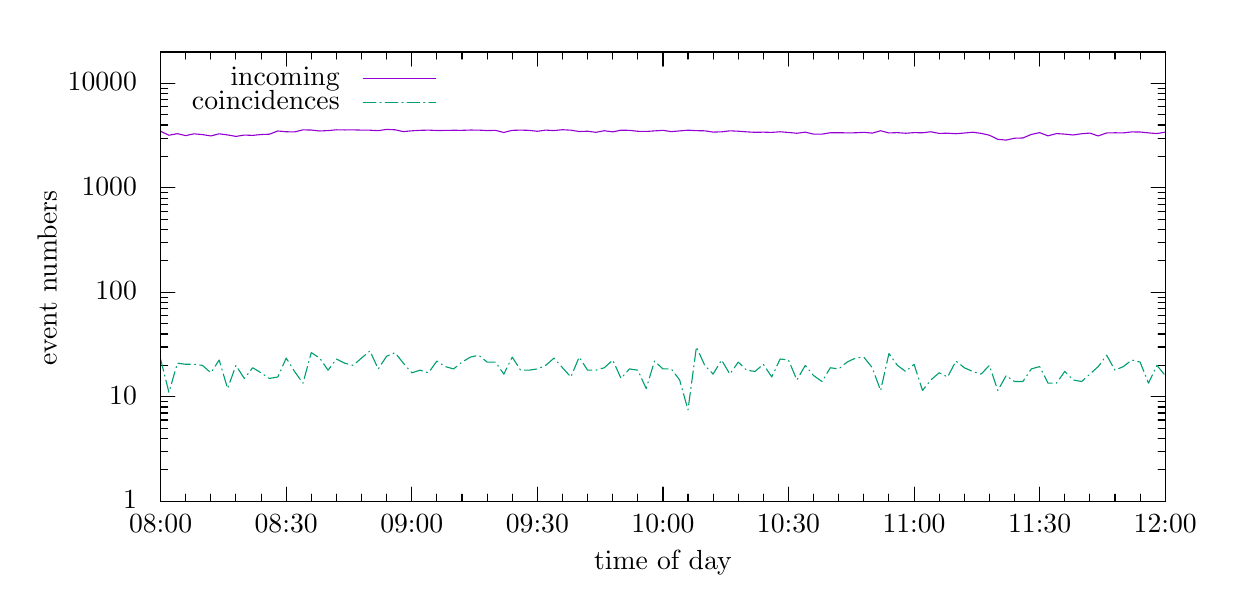
\begin{tikzpicture}[gnuplot]
%% generated with GNUPLOT 5.4p1 (Lua 5.4; terminal rev. Jun 2020, script rev. 114)
%% Mon 19 Jul 2021 16:36:06
\path (0.000,0.000) rectangle (15.000,7.000);
\gpcolor{color=gp lt color border}
\gpsetlinetype{gp lt border}
\gpsetdashtype{gp dt solid}
\gpsetlinewidth{1.00}
\draw[gp path] (1.688,0.985)--(1.868,0.985);
\draw[gp path] (14.447,0.985)--(14.267,0.985);
\node[gp node right] at (1.504,0.985) {$1$};
\draw[gp path] (1.688,1.384)--(1.778,1.384);
\draw[gp path] (14.447,1.384)--(14.357,1.384);
\draw[gp path] (1.688,1.618)--(1.778,1.618);
\draw[gp path] (14.447,1.618)--(14.357,1.618);
\draw[gp path] (1.688,1.784)--(1.778,1.784);
\draw[gp path] (14.447,1.784)--(14.357,1.784);
\draw[gp path] (1.688,1.912)--(1.778,1.912);
\draw[gp path] (14.447,1.912)--(14.357,1.912);
\draw[gp path] (1.688,2.017)--(1.778,2.017);
\draw[gp path] (14.447,2.017)--(14.357,2.017);
\draw[gp path] (1.688,2.106)--(1.778,2.106);
\draw[gp path] (14.447,2.106)--(14.357,2.106);
\draw[gp path] (1.688,2.183)--(1.778,2.183);
\draw[gp path] (14.447,2.183)--(14.357,2.183);
\draw[gp path] (1.688,2.251)--(1.778,2.251);
\draw[gp path] (14.447,2.251)--(14.357,2.251);
\draw[gp path] (1.688,2.312)--(1.868,2.312);
\draw[gp path] (14.447,2.312)--(14.267,2.312);
\node[gp node right] at (1.504,2.312) {$10$};
\draw[gp path] (1.688,2.711)--(1.778,2.711);
\draw[gp path] (14.447,2.711)--(14.357,2.711);
\draw[gp path] (1.688,2.945)--(1.778,2.945);
\draw[gp path] (14.447,2.945)--(14.357,2.945);
\draw[gp path] (1.688,3.110)--(1.778,3.110);
\draw[gp path] (14.447,3.110)--(14.357,3.110);
\draw[gp path] (1.688,3.239)--(1.778,3.239);
\draw[gp path] (14.447,3.239)--(14.357,3.239);
\draw[gp path] (1.688,3.344)--(1.778,3.344);
\draw[gp path] (14.447,3.344)--(14.357,3.344);
\draw[gp path] (1.688,3.433)--(1.778,3.433);
\draw[gp path] (14.447,3.433)--(14.357,3.433);
\draw[gp path] (1.688,3.510)--(1.778,3.510);
\draw[gp path] (14.447,3.510)--(14.357,3.510);
\draw[gp path] (1.688,3.578)--(1.778,3.578);
\draw[gp path] (14.447,3.578)--(14.357,3.578);
\draw[gp path] (1.688,3.638)--(1.868,3.638);
\draw[gp path] (14.447,3.638)--(14.267,3.638);
\node[gp node right] at (1.504,3.638) {$100$};
\draw[gp path] (1.688,4.038)--(1.778,4.038);
\draw[gp path] (14.447,4.038)--(14.357,4.038);
\draw[gp path] (1.688,4.271)--(1.778,4.271);
\draw[gp path] (14.447,4.271)--(14.357,4.271);
\draw[gp path] (1.688,4.437)--(1.778,4.437);
\draw[gp path] (14.447,4.437)--(14.357,4.437);
\draw[gp path] (1.688,4.566)--(1.778,4.566);
\draw[gp path] (14.447,4.566)--(14.357,4.566);
\draw[gp path] (1.688,4.671)--(1.778,4.671);
\draw[gp path] (14.447,4.671)--(14.357,4.671);
\draw[gp path] (1.688,4.759)--(1.778,4.759);
\draw[gp path] (14.447,4.759)--(14.357,4.759);
\draw[gp path] (1.688,4.836)--(1.778,4.836);
\draw[gp path] (14.447,4.836)--(14.357,4.836);
\draw[gp path] (1.688,4.904)--(1.778,4.904);
\draw[gp path] (14.447,4.904)--(14.357,4.904);
\draw[gp path] (1.688,4.965)--(1.868,4.965);
\draw[gp path] (14.447,4.965)--(14.267,4.965);
\node[gp node right] at (1.504,4.965) {$1000$};
\draw[gp path] (1.688,5.364)--(1.778,5.364);
\draw[gp path] (14.447,5.364)--(14.357,5.364);
\draw[gp path] (1.688,5.598)--(1.778,5.598);
\draw[gp path] (14.447,5.598)--(14.357,5.598);
\draw[gp path] (1.688,5.764)--(1.778,5.764);
\draw[gp path] (14.447,5.764)--(14.357,5.764);
\draw[gp path] (1.688,5.892)--(1.778,5.892);
\draw[gp path] (14.447,5.892)--(14.357,5.892);
\draw[gp path] (1.688,5.997)--(1.778,5.997);
\draw[gp path] (14.447,5.997)--(14.357,5.997);
\draw[gp path] (1.688,6.086)--(1.778,6.086);
\draw[gp path] (14.447,6.086)--(14.357,6.086);
\draw[gp path] (1.688,6.163)--(1.778,6.163);
\draw[gp path] (14.447,6.163)--(14.357,6.163);
\draw[gp path] (1.688,6.231)--(1.778,6.231);
\draw[gp path] (14.447,6.231)--(14.357,6.231);
\draw[gp path] (1.688,6.292)--(1.868,6.292);
\draw[gp path] (14.447,6.292)--(14.267,6.292);
\node[gp node right] at (1.504,6.292) {$10000$};
\draw[gp path] (1.688,6.691)--(1.778,6.691);
\draw[gp path] (14.447,6.691)--(14.357,6.691);
\draw[gp path] (1.688,0.985)--(1.688,1.165);
\draw[gp path] (1.688,6.691)--(1.688,6.511);
\node[gp node center] at (1.688,0.677) {08:00};
\draw[gp path] (2.007,0.985)--(2.007,1.075);
\draw[gp path] (2.007,6.691)--(2.007,6.601);
\draw[gp path] (2.326,0.985)--(2.326,1.075);
\draw[gp path] (2.326,6.691)--(2.326,6.601);
\draw[gp path] (2.645,0.985)--(2.645,1.075);
\draw[gp path] (2.645,6.691)--(2.645,6.601);
\draw[gp path] (2.964,0.985)--(2.964,1.075);
\draw[gp path] (2.964,6.691)--(2.964,6.601);
\draw[gp path] (3.283,0.985)--(3.283,1.165);
\draw[gp path] (3.283,6.691)--(3.283,6.511);
\node[gp node center] at (3.283,0.677) {08:30};
\draw[gp path] (3.602,0.985)--(3.602,1.075);
\draw[gp path] (3.602,6.691)--(3.602,6.601);
\draw[gp path] (3.921,0.985)--(3.921,1.075);
\draw[gp path] (3.921,6.691)--(3.921,6.601);
\draw[gp path] (4.240,0.985)--(4.240,1.075);
\draw[gp path] (4.240,6.691)--(4.240,6.601);
\draw[gp path] (4.559,0.985)--(4.559,1.075);
\draw[gp path] (4.559,6.691)--(4.559,6.601);
\draw[gp path] (4.878,0.985)--(4.878,1.165);
\draw[gp path] (4.878,6.691)--(4.878,6.511);
\node[gp node center] at (4.878,0.677) {09:00};
\draw[gp path] (5.197,0.985)--(5.197,1.075);
\draw[gp path] (5.197,6.691)--(5.197,6.601);
\draw[gp path] (5.516,0.985)--(5.516,1.075);
\draw[gp path] (5.516,6.691)--(5.516,6.601);
\draw[gp path] (5.835,0.985)--(5.835,1.075);
\draw[gp path] (5.835,6.691)--(5.835,6.601);
\draw[gp path] (6.154,0.985)--(6.154,1.075);
\draw[gp path] (6.154,6.691)--(6.154,6.601);
\draw[gp path] (6.473,0.985)--(6.473,1.165);
\draw[gp path] (6.473,6.691)--(6.473,6.511);
\node[gp node center] at (6.473,0.677) {09:30};
\draw[gp path] (6.792,0.985)--(6.792,1.075);
\draw[gp path] (6.792,6.691)--(6.792,6.601);
\draw[gp path] (7.111,0.985)--(7.111,1.075);
\draw[gp path] (7.111,6.691)--(7.111,6.601);
\draw[gp path] (7.430,0.985)--(7.430,1.075);
\draw[gp path] (7.430,6.691)--(7.430,6.601);
\draw[gp path] (7.749,0.985)--(7.749,1.075);
\draw[gp path] (7.749,6.691)--(7.749,6.601);
\draw[gp path] (8.068,0.985)--(8.068,1.165);
\draw[gp path] (8.068,6.691)--(8.068,6.511);
\node[gp node center] at (8.068,0.677) {10:00};
\draw[gp path] (8.386,0.985)--(8.386,1.075);
\draw[gp path] (8.386,6.691)--(8.386,6.601);
\draw[gp path] (8.705,0.985)--(8.705,1.075);
\draw[gp path] (8.705,6.691)--(8.705,6.601);
\draw[gp path] (9.024,0.985)--(9.024,1.075);
\draw[gp path] (9.024,6.691)--(9.024,6.601);
\draw[gp path] (9.343,0.985)--(9.343,1.075);
\draw[gp path] (9.343,6.691)--(9.343,6.601);
\draw[gp path] (9.662,0.985)--(9.662,1.165);
\draw[gp path] (9.662,6.691)--(9.662,6.511);
\node[gp node center] at (9.662,0.677) {10:30};
\draw[gp path] (9.981,0.985)--(9.981,1.075);
\draw[gp path] (9.981,6.691)--(9.981,6.601);
\draw[gp path] (10.300,0.985)--(10.300,1.075);
\draw[gp path] (10.300,6.691)--(10.300,6.601);
\draw[gp path] (10.619,0.985)--(10.619,1.075);
\draw[gp path] (10.619,6.691)--(10.619,6.601);
\draw[gp path] (10.938,0.985)--(10.938,1.075);
\draw[gp path] (10.938,6.691)--(10.938,6.601);
\draw[gp path] (11.257,0.985)--(11.257,1.165);
\draw[gp path] (11.257,6.691)--(11.257,6.511);
\node[gp node center] at (11.257,0.677) {11:00};
\draw[gp path] (11.576,0.985)--(11.576,1.075);
\draw[gp path] (11.576,6.691)--(11.576,6.601);
\draw[gp path] (11.895,0.985)--(11.895,1.075);
\draw[gp path] (11.895,6.691)--(11.895,6.601);
\draw[gp path] (12.214,0.985)--(12.214,1.075);
\draw[gp path] (12.214,6.691)--(12.214,6.601);
\draw[gp path] (12.533,0.985)--(12.533,1.075);
\draw[gp path] (12.533,6.691)--(12.533,6.601);
\draw[gp path] (12.852,0.985)--(12.852,1.165);
\draw[gp path] (12.852,6.691)--(12.852,6.511);
\node[gp node center] at (12.852,0.677) {11:30};
\draw[gp path] (13.171,0.985)--(13.171,1.075);
\draw[gp path] (13.171,6.691)--(13.171,6.601);
\draw[gp path] (13.490,0.985)--(13.490,1.075);
\draw[gp path] (13.490,6.691)--(13.490,6.601);
\draw[gp path] (13.809,0.985)--(13.809,1.075);
\draw[gp path] (13.809,6.691)--(13.809,6.601);
\draw[gp path] (14.128,0.985)--(14.128,1.075);
\draw[gp path] (14.128,6.691)--(14.128,6.601);
\draw[gp path] (14.447,0.985)--(14.447,1.165);
\draw[gp path] (14.447,6.691)--(14.447,6.511);
\node[gp node center] at (14.447,0.677) {12:00};
\draw[gp path] (1.688,6.691)--(1.688,0.985)--(14.447,0.985)--(14.447,6.691)--cycle;
\node[gp node center,rotate=-270] at (0.292,3.838) {event numbers};
\node[gp node center] at (8.067,0.215) {time of day};
\node[gp node right] at (4.080,6.357) {incoming};
\gpcolor{rgb color={0.580,0.000,0.827}}
\draw[gp path] (4.264,6.357)--(5.180,6.357);
\draw[gp path] (1.688,5.684)--(1.794,5.634)--(1.901,5.654)--(2.007,5.629)--(2.113,5.652)%
  --(2.220,5.642)--(2.326,5.625)--(2.432,5.652)--(2.539,5.638)--(2.645,5.619)--(2.751,5.636)%
  --(2.858,5.632)--(2.964,5.643)--(3.070,5.647)--(3.177,5.688)--(3.283,5.678)--(3.389,5.676)%
  --(3.496,5.702)--(3.602,5.700)--(3.708,5.688)--(3.815,5.693)--(3.921,5.703)--(4.027,5.701)%
  --(4.133,5.702)--(4.240,5.699)--(4.346,5.698)--(4.452,5.692)--(4.559,5.708)--(4.665,5.703)%
  --(4.771,5.680)--(4.878,5.690)--(4.984,5.696)--(5.090,5.699)--(5.197,5.694)--(5.303,5.695)%
  --(5.409,5.697)--(5.516,5.696)--(5.622,5.700)--(5.728,5.699)--(5.835,5.693)--(5.941,5.696)%
  --(6.047,5.669)--(6.154,5.696)--(6.260,5.699)--(6.366,5.696)--(6.473,5.684)--(6.579,5.699)%
  --(6.685,5.693)--(6.792,5.704)--(6.898,5.698)--(7.004,5.681)--(7.111,5.685)--(7.217,5.671)%
  --(7.323,5.691)--(7.430,5.677)--(7.536,5.698)--(7.642,5.696)--(7.749,5.684)--(7.855,5.682)%
  --(7.961,5.689)--(8.068,5.696)--(8.174,5.680)--(8.280,5.689)--(8.386,5.698)--(8.493,5.692)%
  --(8.599,5.690)--(8.705,5.674)--(8.812,5.677)--(8.918,5.690)--(9.024,5.685)--(9.131,5.677)%
  --(9.237,5.671)--(9.343,5.673)--(9.450,5.670)--(9.556,5.678)--(9.662,5.669)--(9.769,5.659)%
  --(9.875,5.673)--(9.981,5.648)--(10.088,5.648)--(10.194,5.666)--(10.300,5.666)--(10.407,5.664)%
  --(10.513,5.665)--(10.619,5.671)--(10.726,5.661)--(10.832,5.691)--(10.938,5.663)--(11.045,5.667)%
  --(11.151,5.659)--(11.257,5.667)--(11.364,5.665)--(11.470,5.678)--(11.576,5.657)--(11.683,5.660)%
  --(11.789,5.653)--(11.895,5.662)--(12.002,5.672)--(12.108,5.658)--(12.214,5.634)--(12.321,5.582)%
  --(12.427,5.572)--(12.533,5.596)--(12.639,5.599)--(12.746,5.644)--(12.852,5.667)--(12.958,5.626)%
  --(13.065,5.655)--(13.171,5.648)--(13.277,5.637)--(13.384,5.653)--(13.490,5.661)--(13.596,5.625)%
  --(13.703,5.663)--(13.809,5.665)--(13.915,5.664)--(14.022,5.676)--(14.128,5.675)--(14.234,5.664)%
  --(14.341,5.655)--(14.447,5.673);
\gpcolor{color=gp lt color border}
\node[gp node right] at (4.080,6.049) {coincidences};
\gpcolor{rgb color={0.000,0.620,0.451}}
\gpsetdashtype{gp dt 5}
\draw[gp path] (4.264,6.049)--(5.180,6.049);
\draw[gp path] (1.688,2.792)--(1.794,2.367)--(1.901,2.739)--(2.007,2.725)--(2.113,2.725)%
  --(2.220,2.711)--(2.326,2.617)--(2.432,2.779)--(2.539,2.417)--(2.645,2.711)--(2.751,2.545)%
  --(2.858,2.681)--(2.964,2.617)--(3.070,2.545)--(3.177,2.564)--(3.283,2.804)--(3.389,2.634)%
  --(3.496,2.485)--(3.602,2.873)--(3.708,2.804)--(3.815,2.650)--(3.921,2.792)--(4.027,2.739)%
  --(4.133,2.711)--(4.240,2.804)--(4.346,2.895)--(4.452,2.666)--(4.559,2.828)--(4.665,2.873)%
  --(4.771,2.739)--(4.878,2.617)--(4.984,2.650)--(5.090,2.617)--(5.197,2.766)--(5.303,2.696)%
  --(5.409,2.666)--(5.516,2.753)--(5.622,2.816)--(5.728,2.840)--(5.835,2.753)--(5.941,2.753)%
  --(6.047,2.600)--(6.154,2.816)--(6.260,2.650)--(6.366,2.650)--(6.473,2.666)--(6.579,2.711)%
  --(6.685,2.804)--(6.792,2.681)--(6.898,2.564)--(7.004,2.816)--(7.111,2.650)--(7.217,2.650)%
  --(7.323,2.681)--(7.430,2.779)--(7.536,2.545)--(7.642,2.666)--(7.749,2.650)--(7.855,2.417)%
  --(7.961,2.766)--(8.068,2.666)--(8.174,2.666)--(8.280,2.526)--(8.386,2.146)--(8.493,2.945)%
  --(8.599,2.711)--(8.705,2.600)--(8.812,2.779)--(8.918,2.600)--(9.024,2.753)--(9.131,2.650)%
  --(9.237,2.634)--(9.343,2.725)--(9.450,2.564)--(9.556,2.792)--(9.662,2.779)--(9.769,2.526)%
  --(9.875,2.711)--(9.981,2.582)--(10.088,2.506)--(10.194,2.681)--(10.300,2.666)--(10.407,2.753)%
  --(10.513,2.804)--(10.619,2.816)--(10.726,2.681)--(10.832,2.392)--(10.938,2.862)--(11.045,2.711)%
  --(11.151,2.634)--(11.257,2.725)--(11.364,2.392)--(11.470,2.526)--(11.576,2.617)--(11.683,2.564)%
  --(11.789,2.766)--(11.895,2.681)--(12.002,2.634)--(12.108,2.600)--(12.214,2.711)--(12.321,2.392)%
  --(12.427,2.582)--(12.533,2.506)--(12.639,2.506)--(12.746,2.666)--(12.852,2.696)--(12.958,2.485)%
  --(13.065,2.485)--(13.171,2.634)--(13.277,2.526)--(13.384,2.506)--(13.490,2.600)--(13.596,2.696)%
  --(13.703,2.840)--(13.809,2.650)--(13.915,2.696)--(14.022,2.779)--(14.128,2.753)--(14.234,2.485)%
  --(14.341,2.711)--(14.447,2.582);
\gpcolor{color=gp lt color border}
\gpsetdashtype{gp dt solid}
\draw[gp path] (1.688,6.691)--(1.688,0.985)--(14.447,0.985)--(14.447,6.691)--cycle;
%% coordinates of the plot area
\gpdefrectangularnode{gp plot 1}{\pgfpoint{1.688cm}{0.985cm}}{\pgfpoint{14.447cm}{6.691cm}}
\end{tikzpicture}
%% gnuplot variables

\caption{Example of incoming raw and outgoing coincidence event rate over $4\,\text{hour}$ period}
\label{fig:rates-example}
\end{figure}

\begin{figure}[ht!]
	\centering
	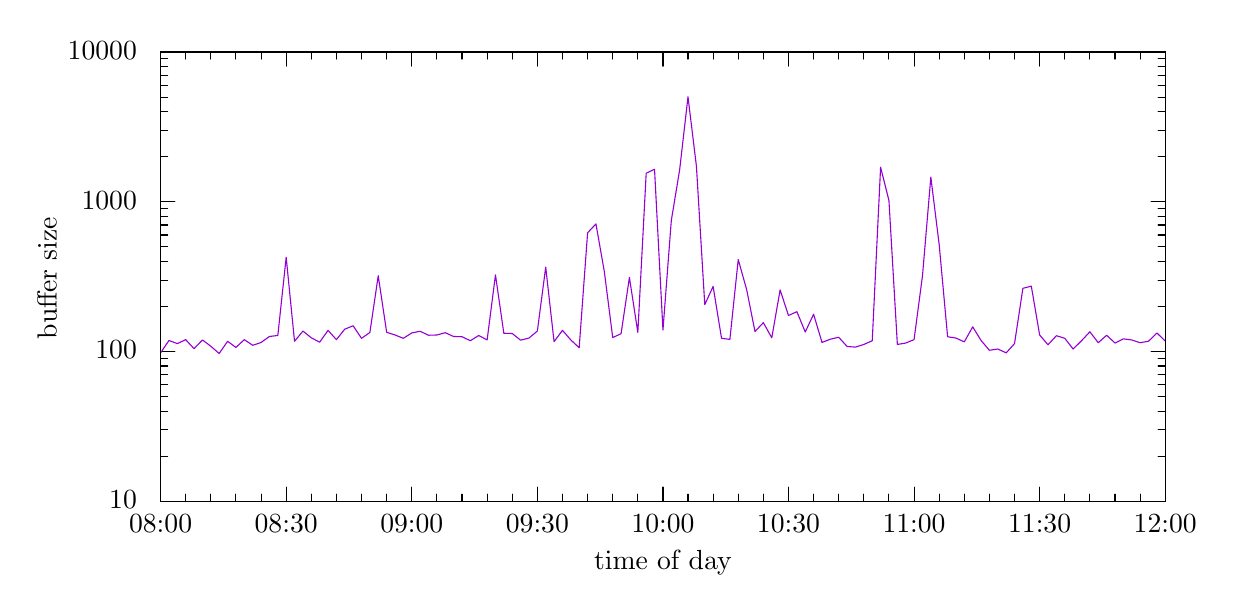
\begin{tikzpicture}[gnuplot]
%% generated with GNUPLOT 5.4p1 (Lua 5.4; terminal rev. Jun 2020, script rev. 114)
%% Mon 19 Jul 2021 16:30:23
\path (0.000,0.000) rectangle (15.000,7.000);
\gpcolor{color=gp lt color border}
\gpsetlinetype{gp lt border}
\gpsetdashtype{gp dt solid}
\gpsetlinewidth{1.00}
\draw[gp path] (1.688,0.985)--(1.868,0.985);
\draw[gp path] (14.447,0.985)--(14.267,0.985);
\node[gp node right] at (1.504,0.985) {$10$};
\draw[gp path] (1.688,1.558)--(1.778,1.558);
\draw[gp path] (14.447,1.558)--(14.357,1.558);
\draw[gp path] (1.688,1.892)--(1.778,1.892);
\draw[gp path] (14.447,1.892)--(14.357,1.892);
\draw[gp path] (1.688,2.130)--(1.778,2.130);
\draw[gp path] (14.447,2.130)--(14.357,2.130);
\draw[gp path] (1.688,2.314)--(1.778,2.314);
\draw[gp path] (14.447,2.314)--(14.357,2.314);
\draw[gp path] (1.688,2.465)--(1.778,2.465);
\draw[gp path] (14.447,2.465)--(14.357,2.465);
\draw[gp path] (1.688,2.592)--(1.778,2.592);
\draw[gp path] (14.447,2.592)--(14.357,2.592);
\draw[gp path] (1.688,2.703)--(1.778,2.703);
\draw[gp path] (14.447,2.703)--(14.357,2.703);
\draw[gp path] (1.688,2.800)--(1.778,2.800);
\draw[gp path] (14.447,2.800)--(14.357,2.800);
\draw[gp path] (1.688,2.887)--(1.868,2.887);
\draw[gp path] (14.447,2.887)--(14.267,2.887);
\node[gp node right] at (1.504,2.887) {$100$};
\draw[gp path] (1.688,3.460)--(1.778,3.460);
\draw[gp path] (14.447,3.460)--(14.357,3.460);
\draw[gp path] (1.688,3.794)--(1.778,3.794);
\draw[gp path] (14.447,3.794)--(14.357,3.794);
\draw[gp path] (1.688,4.032)--(1.778,4.032);
\draw[gp path] (14.447,4.032)--(14.357,4.032);
\draw[gp path] (1.688,4.216)--(1.778,4.216);
\draw[gp path] (14.447,4.216)--(14.357,4.216);
\draw[gp path] (1.688,4.367)--(1.778,4.367);
\draw[gp path] (14.447,4.367)--(14.357,4.367);
\draw[gp path] (1.688,4.494)--(1.778,4.494);
\draw[gp path] (14.447,4.494)--(14.357,4.494);
\draw[gp path] (1.688,4.605)--(1.778,4.605);
\draw[gp path] (14.447,4.605)--(14.357,4.605);
\draw[gp path] (1.688,4.702)--(1.778,4.702);
\draw[gp path] (14.447,4.702)--(14.357,4.702);
\draw[gp path] (1.688,4.789)--(1.868,4.789);
\draw[gp path] (14.447,4.789)--(14.267,4.789);
\node[gp node right] at (1.504,4.789) {$1000$};
\draw[gp path] (1.688,5.362)--(1.778,5.362);
\draw[gp path] (14.447,5.362)--(14.357,5.362);
\draw[gp path] (1.688,5.696)--(1.778,5.696);
\draw[gp path] (14.447,5.696)--(14.357,5.696);
\draw[gp path] (1.688,5.934)--(1.778,5.934);
\draw[gp path] (14.447,5.934)--(14.357,5.934);
\draw[gp path] (1.688,6.118)--(1.778,6.118);
\draw[gp path] (14.447,6.118)--(14.357,6.118);
\draw[gp path] (1.688,6.269)--(1.778,6.269);
\draw[gp path] (14.447,6.269)--(14.357,6.269);
\draw[gp path] (1.688,6.396)--(1.778,6.396);
\draw[gp path] (14.447,6.396)--(14.357,6.396);
\draw[gp path] (1.688,6.507)--(1.778,6.507);
\draw[gp path] (14.447,6.507)--(14.357,6.507);
\draw[gp path] (1.688,6.604)--(1.778,6.604);
\draw[gp path] (14.447,6.604)--(14.357,6.604);
\draw[gp path] (1.688,6.691)--(1.868,6.691);
\draw[gp path] (14.447,6.691)--(14.267,6.691);
\node[gp node right] at (1.504,6.691) {$10000$};
\draw[gp path] (1.688,0.985)--(1.688,1.165);
\draw[gp path] (1.688,6.691)--(1.688,6.511);
\node[gp node center] at (1.688,0.677) {08:00};
\draw[gp path] (2.007,0.985)--(2.007,1.075);
\draw[gp path] (2.007,6.691)--(2.007,6.601);
\draw[gp path] (2.326,0.985)--(2.326,1.075);
\draw[gp path] (2.326,6.691)--(2.326,6.601);
\draw[gp path] (2.645,0.985)--(2.645,1.075);
\draw[gp path] (2.645,6.691)--(2.645,6.601);
\draw[gp path] (2.964,0.985)--(2.964,1.075);
\draw[gp path] (2.964,6.691)--(2.964,6.601);
\draw[gp path] (3.283,0.985)--(3.283,1.165);
\draw[gp path] (3.283,6.691)--(3.283,6.511);
\node[gp node center] at (3.283,0.677) {08:30};
\draw[gp path] (3.602,0.985)--(3.602,1.075);
\draw[gp path] (3.602,6.691)--(3.602,6.601);
\draw[gp path] (3.921,0.985)--(3.921,1.075);
\draw[gp path] (3.921,6.691)--(3.921,6.601);
\draw[gp path] (4.240,0.985)--(4.240,1.075);
\draw[gp path] (4.240,6.691)--(4.240,6.601);
\draw[gp path] (4.559,0.985)--(4.559,1.075);
\draw[gp path] (4.559,6.691)--(4.559,6.601);
\draw[gp path] (4.878,0.985)--(4.878,1.165);
\draw[gp path] (4.878,6.691)--(4.878,6.511);
\node[gp node center] at (4.878,0.677) {09:00};
\draw[gp path] (5.197,0.985)--(5.197,1.075);
\draw[gp path] (5.197,6.691)--(5.197,6.601);
\draw[gp path] (5.516,0.985)--(5.516,1.075);
\draw[gp path] (5.516,6.691)--(5.516,6.601);
\draw[gp path] (5.835,0.985)--(5.835,1.075);
\draw[gp path] (5.835,6.691)--(5.835,6.601);
\draw[gp path] (6.154,0.985)--(6.154,1.075);
\draw[gp path] (6.154,6.691)--(6.154,6.601);
\draw[gp path] (6.473,0.985)--(6.473,1.165);
\draw[gp path] (6.473,6.691)--(6.473,6.511);
\node[gp node center] at (6.473,0.677) {09:30};
\draw[gp path] (6.792,0.985)--(6.792,1.075);
\draw[gp path] (6.792,6.691)--(6.792,6.601);
\draw[gp path] (7.111,0.985)--(7.111,1.075);
\draw[gp path] (7.111,6.691)--(7.111,6.601);
\draw[gp path] (7.430,0.985)--(7.430,1.075);
\draw[gp path] (7.430,6.691)--(7.430,6.601);
\draw[gp path] (7.749,0.985)--(7.749,1.075);
\draw[gp path] (7.749,6.691)--(7.749,6.601);
\draw[gp path] (8.068,0.985)--(8.068,1.165);
\draw[gp path] (8.068,6.691)--(8.068,6.511);
\node[gp node center] at (8.068,0.677) {10:00};
\draw[gp path] (8.386,0.985)--(8.386,1.075);
\draw[gp path] (8.386,6.691)--(8.386,6.601);
\draw[gp path] (8.705,0.985)--(8.705,1.075);
\draw[gp path] (8.705,6.691)--(8.705,6.601);
\draw[gp path] (9.024,0.985)--(9.024,1.075);
\draw[gp path] (9.024,6.691)--(9.024,6.601);
\draw[gp path] (9.343,0.985)--(9.343,1.075);
\draw[gp path] (9.343,6.691)--(9.343,6.601);
\draw[gp path] (9.662,0.985)--(9.662,1.165);
\draw[gp path] (9.662,6.691)--(9.662,6.511);
\node[gp node center] at (9.662,0.677) {10:30};
\draw[gp path] (9.981,0.985)--(9.981,1.075);
\draw[gp path] (9.981,6.691)--(9.981,6.601);
\draw[gp path] (10.300,0.985)--(10.300,1.075);
\draw[gp path] (10.300,6.691)--(10.300,6.601);
\draw[gp path] (10.619,0.985)--(10.619,1.075);
\draw[gp path] (10.619,6.691)--(10.619,6.601);
\draw[gp path] (10.938,0.985)--(10.938,1.075);
\draw[gp path] (10.938,6.691)--(10.938,6.601);
\draw[gp path] (11.257,0.985)--(11.257,1.165);
\draw[gp path] (11.257,6.691)--(11.257,6.511);
\node[gp node center] at (11.257,0.677) {11:00};
\draw[gp path] (11.576,0.985)--(11.576,1.075);
\draw[gp path] (11.576,6.691)--(11.576,6.601);
\draw[gp path] (11.895,0.985)--(11.895,1.075);
\draw[gp path] (11.895,6.691)--(11.895,6.601);
\draw[gp path] (12.214,0.985)--(12.214,1.075);
\draw[gp path] (12.214,6.691)--(12.214,6.601);
\draw[gp path] (12.533,0.985)--(12.533,1.075);
\draw[gp path] (12.533,6.691)--(12.533,6.601);
\draw[gp path] (12.852,0.985)--(12.852,1.165);
\draw[gp path] (12.852,6.691)--(12.852,6.511);
\node[gp node center] at (12.852,0.677) {11:30};
\draw[gp path] (13.171,0.985)--(13.171,1.075);
\draw[gp path] (13.171,6.691)--(13.171,6.601);
\draw[gp path] (13.490,0.985)--(13.490,1.075);
\draw[gp path] (13.490,6.691)--(13.490,6.601);
\draw[gp path] (13.809,0.985)--(13.809,1.075);
\draw[gp path] (13.809,6.691)--(13.809,6.601);
\draw[gp path] (14.128,0.985)--(14.128,1.075);
\draw[gp path] (14.128,6.691)--(14.128,6.601);
\draw[gp path] (14.447,0.985)--(14.447,1.165);
\draw[gp path] (14.447,6.691)--(14.447,6.511);
\node[gp node center] at (14.447,0.677) {12:00};
\draw[gp path] (1.688,6.691)--(1.688,0.985)--(14.447,0.985)--(14.447,6.691)--cycle;
\node[gp node center,rotate=-270] at (0.292,3.838) {buffer size};
\node[gp node center] at (8.067,0.215) {time of day};
\gpcolor{rgb color={0.580,0.000,0.827}}
\draw[gp path] (1.688,2.870)--(1.794,3.027)--(1.901,2.988)--(2.007,3.038)--(2.113,2.923)%
  --(2.220,3.034)--(2.326,2.954)--(2.432,2.862)--(2.539,3.017)--(2.645,2.939)--(2.751,3.038)%
  --(2.858,2.966)--(2.964,3.002)--(3.070,3.078)--(3.177,3.091)--(3.283,4.084)--(3.389,3.017)%
  --(3.496,3.147)--(3.602,3.061)--(3.708,3.006)--(3.815,3.156)--(3.921,3.038)--(4.027,3.171)%
  --(4.133,3.214)--(4.240,3.055)--(4.346,3.129)--(4.452,3.849)--(4.559,3.132)--(4.665,3.097)%
  --(4.771,3.055)--(4.878,3.123)--(4.984,3.144)--(5.090,3.094)--(5.197,3.097)--(5.303,3.126)%
  --(5.409,3.078)--(5.516,3.075)--(5.622,3.024)--(5.728,3.091)--(5.835,3.034)--(5.941,3.861)%
  --(6.047,3.119)--(6.154,3.116)--(6.260,3.031)--(6.366,3.058)--(6.473,3.147)--(6.579,3.959)%
  --(6.685,3.013)--(6.792,3.156)--(6.898,3.034)--(7.004,2.935)--(7.111,4.395)--(7.217,4.508)%
  --(7.323,3.905)--(7.430,3.065)--(7.536,3.113)--(7.642,3.828)--(7.749,3.129)--(7.855,5.151)%
  --(7.961,5.202)--(8.068,3.159)--(8.174,4.550)--(8.280,5.195)--(8.386,6.122)--(8.493,5.241)%
  --(8.599,3.482)--(8.705,3.714)--(8.812,3.055)--(8.918,3.041)--(9.024,4.055)--(9.131,3.673)%
  --(9.237,3.141)--(9.343,3.254)--(9.450,3.061)--(9.556,3.670)--(9.662,3.345)--(9.769,3.393)%
  --(9.875,3.135)--(9.981,3.361)--(10.088,3.002)--(10.194,3.044)--(10.300,3.068)--(10.407,2.951)%
  --(10.513,2.943)--(10.619,2.977)--(10.726,3.024)--(10.832,5.228)--(10.938,4.805)--(11.045,2.977)%
  --(11.151,2.995)--(11.257,3.038)--(11.364,3.849)--(11.470,5.102)--(11.576,4.245)--(11.683,3.075)%
  --(11.789,3.058)--(11.895,3.010)--(12.002,3.200)--(12.108,3.027)--(12.214,2.903)--(12.321,2.919)%
  --(12.427,2.870)--(12.533,2.988)--(12.639,3.690)--(12.746,3.717)--(12.852,3.097)--(12.958,2.973)%
  --(13.065,3.088)--(13.171,3.055)--(13.277,2.919)--(13.384,3.024)--(13.490,3.138)--(13.596,2.999)%
  --(13.703,3.094)--(13.809,2.995)--(13.915,3.048)--(14.022,3.034)--(14.128,2.999)--(14.234,3.017)%
  --(14.341,3.123)--(14.447,3.020);
\gpcolor{color=gp lt color border}
\draw[gp path] (1.688,6.691)--(1.688,0.985)--(14.447,0.985)--(14.447,6.691)--cycle;
%% coordinates of the plot area
\gpdefrectangularnode{gp plot 1}{\pgfpoint{1.688cm}{0.985cm}}{\pgfpoint{14.447cm}{6.691cm}}
\end{tikzpicture}
%% gnuplot variables

	\caption{Example of event buffer size over $4\,\text{hour}$ period}
	\label{fig:buffer-example}
\end{figure}
Figures \ref{fig:rates-example} and \ref{fig:buffer-example} show the result of an increased timeout value as shown in the example in figure \ref{fig:timeout-example}. Figure \ref{fig:buffer-example} shows the buffer size rise in direct relation to the increased timeout value just after $10$. This in turn causes a drop immediately followed by an increase in outgoing coincidence events as visible in the green and dashed line in figure \ref{fig:rates-example}. In the same plot, the pink line shows the cumulative incoming events between all detector stations. It is important to note though that the event number is not the event rate directly but the total number of events in a sample interval.
\subsection{Coincidence analysis}\label{subsec:coincidence-s}
The coincidence analysis is used to collect useful statistics mainly about detector station pair coincidence rates and histograms. It receives all coincidence events and has knowledge of all current detector stations. \\
With this information it creates a graph of all detector pairs where it tracks the event times and numbers for each pair. Though due to the large number of possible pairs in the number of detector stations, this needs to be done carefully in order to not use too much system memory. The number of pairs out of $n$ detectors can be calculated through the binomial coefficient which in the specific case for $k = 2$ can be calculated with
\begin{equation}
	{n \choose k} = \frac{n!}{k!\cdot\left(n - k\right)!} = \frac{1}{2}\left(n^2 - n\right) = \Delta_{n-1}.
\end{equation}
Which is the same definition for the number of edges in a complete graph. In memory, this construct can be stored as an upper triangular matrix with no diagonal entries.

Each edge in the graph represents the number of coincidences of the associated detector pair and contains a histogram over a sample interval of $24\,\text{hours}$. After the sample interval is elapsed, all current histograms are stored to the disk and the structure in memory is reset.
\clearpage
\section{Conclusion and outlook}
This thesis described the possibility and implementation of a real-time system to analyse data from a loose network of low-cost scintillator detectors. This approach offers the benefit of being able to pre-filter all incoming data for a first plausibility determination. With this, not every data point needs to be saved and the infrastructure has a lower total load.

At this point in time the application only does the filtering step and discards the raw data. A comparison with simultaneously running post-processing analysis software has shown that the real-time application runs reliable and finds all coincidences. In fact it can be observed that the real-time system detects a larger number of coincidences since the post-processing analysis needs to read and write large amounts to and from a database on execution it creates a substantial load on the system. This leads to data being lost during that time interval since the system cannot handle those loads. The real-time system has no large load spikes so does not lose data the same way. As a backup the raw data is still stored through other means however those have not been necessary so far.

Additional benefits of a real-time system are of visual nature. It allows the real-time visualisation of found coincidences on a map through a website and so can give a visual aid as to the validity of recorded data.


The system functions at a good base level already, though further functionality is planned.
Among the planned improvements is an introspection system with which the application can be monitored in real-time and offer runtime configuration options.

The methods described in \ref{sec:analysis} need to be tested rigorously. They have undergone a basic analysis and have shown to work on a basic level though the reliability is not clear as of yet.

\clearpage

\makeback
\end{document}
